\documentclass[11pt]{article}

\usepackage[utf8]{inputenc}
\usepackage{amsmath,amssymb,amsfonts}%
\usepackage{amsthm}%
\usepackage{graphicx}
\usepackage{geometry}
\usepackage{mathrsfs}%
\usepackage{setspace}
\usepackage{float}
\DeclareMathOperator{\Var}{Var}
\DeclareMathOperator{\Cov}{Cov}
\DeclareMathOperator{\supp}{supp}
\newcommand{\EE}{\mathbb{E}}
\usepackage{booktabs}
\usepackage{enumitem}
\usepackage{caption}      % provides \captionof for non-floating captions

% Force "S" prefix on supplementary figures and tables
\renewcommand{\thefigure}{S\arabic{figure}}
\renewcommand{\thetable}{S\arabic{table}}

\newtheorem{theorem}{Theorem}[section]
\newtheorem{lemma}[theorem]{Lemma}
\newtheorem{proposition}[theorem]{Proposition}
\newtheorem{corollary}[theorem]{Corollary}

\theoremstyle{remark}
\newtheorem{remark}[theorem]{Remark}

\theoremstyle{definition}
\newtheorem{definition}[theorem]{Definition}
\newtheorem{example}[theorem]{Example}

\geometry{margin=1in}
\setstretch{1.2}

\title{\textbf{Supplementary Information for:}\\
Gibbs Manifold Geometry Unifies Neural Variability, Sparseness, and Metabolic Efficiency}

\author{Mingyi Huang, Wei Lin, Anna Wang Roe and Yuguo Yu*}



\date{}

\begin{document}

\maketitle

\tableofcontents

\newpage
\section{Normative Principle: Entropy and Information Maximization under Energy Constraints}

\subsection{Problem setting}

We study the problem of maximizing either the output entropy $H(r)$ or the mutual information $I(s;r)$ over a distribution $p(r)$ supported on $[0,r_{\max}]$, subject to a cost budget. Specifically:
\begin{align}
\begin{split}
\max_{p \in \mathcal{P}} \quad & \Phi(p) \in \{ H(r),\, I(s;r)\}, \\
\text{s.t.}\quad & \mathbb{E}_p[c(r)] \le C, \label{eq:cost-constraint} \\
& \mathrm{supp}(p)\subseteq [0,r_{\max}], \\
& \text{(optional) stationarity and refractoriness constraints (linear)}.
\end{split}
\end{align}
We define
\begin{align}
\mathrm{CV}[p] = \frac{\sqrt{\Var_p(r)}}{\mathbb{E}_p[r]}.
\end{align}

\paragraph{Standing assumptions.}
\begin{enumerate}[label=(A\arabic*)]
  \item $c$ is strictly increasing and strictly convex on $[0,r_{\max}]$;
  \item The feasible set is nonempty, and Slater's condition\footnote{Slater’s condition is a standard regularity condition in convex optimization ensuring strong duality. 
  It requires that there exists at least one strictly feasible distribution $p$ such that $\mathbb{E}_p[c(r)]<C$ and all other inequality constraints are satisfied strictly.} holds for \eqref{eq:cost-constraint};
  \item For the mutual information objective, the conditional law $p(r|s)$ belongs to a regular exponential family with natural parameter depending on $s$, and any additional constraints are linear in $p$.
\end{enumerate}
\subsection{Relationship 1: CV--$\beta$ coupling (general setup)}
\label{sec:cv-beta-general}

We analyze the family of optimal response distributions obtained under the entropy (or information) maximization problem with a metabolic budget, and establish the first structural relationship of the Gibbs manifold: the monotone coupling between the coefficient of variation $\mathrm{CV}$ and the marginal efficiency $\beta$.  Throughout this section we assume (A1)--(A2) from the main text: the cost $c(r)$ is strictly increasing and strictly convex, the feasible set is nonempty, and Slater's condition holds.

\paragraph{Optimality: exponential-family structure.}
The key structural result is that the constrained entropy maximizer is always a Gibbs distribution.

\begin{lemma}[Optimal distribution via KKT]
\label{lem:gibbs}
Under (A1)--(A2), any entropy maximizer supported on $[0,r_{\max}]$ has the form
\begin{align}
p_\beta(r)
= \frac{1}{Z(\beta)}\,\exp\!\bigl(-\beta\,c(r)\bigr)\,
\mathbf{1}_{[0,r_{\max}]}(r), 
\qquad 
Z(\beta)=\int_0^{r_{\max}} e^{-\beta c(r)}\,dr,
\end{align}
for some multiplier $\beta\ge 0$, chosen so that 
$\EE_{p_\beta}[c(r)] = C$ whenever the constraint is active.
Any additional \emph{linear} constraints add linear sufficient statistics in the exponent, preserving exponential-family structure.
\end{lemma}

\begin{proof}
Maximizing 
$H(p)=-\int p\log p$ 
under the normalization and cost constraints yields a concave optimization problem.  
The KKT stationarity condition of the Lagrangian
\(
\mathcal{L}= -\int p\log p
+ \beta\!\Bigl(C-\int c\,p\Bigr)
+ \nu\!\Bigl(1-\int p\Bigr)
\)
implies $\log p(r) = -1-\nu - \beta c(r)$ and hence the claimed form.  
Strict concavity of $H$ ensures uniqueness when the constraint is active.
\end{proof}

\subsubsection{Moment identities along the Gibbs family.}
To characterize how the moments of $p_\beta$ evolve as efficiency increases (i.e.\ as $\beta$ varies), we use the following derivative identity.

\begin{lemma}[Moment derivatives along an exponential family]
\label{lem:moment-deriv}
For any integrable $g$, the expectation $\EE_{p_\beta}[g]$ is differentiable and
\begin{align}
\frac{d}{d\beta}\EE_{p_\beta}[g(r)]
= -\Cov_{p_\beta}\!\bigl(g(r),\,c(r)\bigr).
\end{align}
\end{lemma}

\begin{remark}[Consequences for the partition function]
From the same calculation,
\begin{align}
\frac{d}{d\beta}\log Z(\beta) = -\EE[c],\qquad
\frac{d^2}{d\beta^2}\log Z(\beta) = \Var(c)\ge 0.
\end{align}
Thus $\log Z$ is convex in $\beta$.
\end{remark}

\subsubsection{Derivatives of mean, variance, and CV.}
Applying Lemma~\ref{lem:moment-deriv} to $g(r)=r$ and 
$g(r)=(r-\EE r)^2$ gives
\begin{align}
\frac{d}{d\beta}\EE[r] &= -\Cov(r,c), \\
\frac{d}{d\beta}\Var(r) &= -\Cov\!\bigl((r-\EE r)^2,c(r)\bigr).
\end{align}
If $c$ is increasing and convex, both covariances are strictly positive, so both derivatives are strictly negative.

When $\beta$ is determined by the active budget constraint 
$\EE[c]=C$, we obtain
\begin{align}
\frac{dC}{d\beta} = -\Var(c)<0,
\end{align}
so $\beta$ is strictly decreasing in $C$.  
For any $g$,
\begin{align}
\frac{d}{dC}\EE[g]
= \frac{\Cov(g,c)}{\Var(c)}.
\end{align}

For the coefficient of variation
\(
\mathrm{CV}(\beta)=\sqrt{\Var}/\EE[r],
\)
differentiation yields
\begin{align}
\frac{d}{d\beta}\log\mathrm{CV}
= -\frac{1}{2}\frac{\Cov((r-\EE r)^2,c)}{\Var(r)}
+ \frac{\Cov(r,c)}{\EE[r]}.
\label{eq:dlogcv}
\end{align}
The two covariance terms are both positive; their relative size determines the sign of the derivative.

\subsubsection{Monotonicity of CV along the optimal family.}
We now state the main monotonicity property used throughout the main text.

\begin{theorem}[CV increases with metabolic tightness]
\label{thm:cv-monotone}
Under (A1)--(A2) and a mild covariance domination condition
(Supplementary Proof~\ref{proof:cov-dominate}),
the optimal Gibbs family $p_\beta$ satisfies:
\begin{align}
\beta \uparrow \quad \Longrightarrow \quad
\mathrm{CV}[p_\beta] \uparrow ,
\qquad\text{equivalently,}\qquad
C \uparrow \quad \Longrightarrow \quad \mathrm{CV}[p_\beta] \downarrow .
\end{align}
That is, $\mathrm{CV}$ is a strictly increasing function of $\beta$ (and strictly decreasing in the budget $C$).
\end{theorem}

\begin{proof}
Lemma~\ref{lem:gibbs} and Lemma~\ref{lem:moment-deriv} imply that 
$\EE[r]$, $\Var(r)$, and $C$ all decrease with $\beta$.  
Using \eqref{eq:dlogcv}, monotonicity follows once the linear covariance term dominates the quadratic one, which is shown under the stated domination condition.
\end{proof}

\subsubsection{Consequences for entropy and information.}

\begin{proposition}[Variation of $H$, $I$, and ICE along the Gibbs manifold]
\label{prop:H-I-vs-CV}
Along the optimal family $p_\beta$ parameterized by $\beta\in(0,\infty)$:
\begin{enumerate}[label=(\alph*)]
\item $H(r)$ strictly \emph{decreases} with $\beta$ (tighter budgets leave less room for entropy), and hence by Theorem~\ref{thm:cv-monotone} strictly \emph{decreases} with $\mathrm{CV}[p_\beta]$.
\item If the noise entropy $H(r|s)$ is independent of $p(r)$
(e.g.\ additive noise with fixed entropy),
then the mutual information $I(s;r)$ also strictly decreases with $\mathrm{CV}[p_\beta]$.
\item The \emph{information--cost efficiency} $\mathrm{ICE}(\beta)=H(\beta)/C(\beta)$ behaves in the opposite direction: whenever $\log Z(\beta)>0$ (equivalently, whenever the chosen information convention satisfies $H^\star(0)\ge 0$), $\mathrm{ICE}$ strictly \emph{increases} with $\mathrm{CV}[p_\beta]$.  This is the regime relevant to the main text; a full analysis appears in Sections~\ref{sec:marginal-average-coupling}--\ref{sec:ice-cv-unified}.
\end{enumerate}
\end{proposition}

\begin{proof}
(a) Using the Gibbs form, $H(\beta)=\beta C(\beta)+\log Z(\beta)$, so
\(
dH/d\beta = C + \beta\,(dC/d\beta) + d\log Z/d\beta = C - \beta\Var(c) - C = -\beta\Var(c) < 0
\)
for $\beta>0$.  Since $d\,\mathrm{CV}/d\beta>0$ (Theorem~\ref{thm:cv-monotone}), $H$ strictly decreases with $\mathrm{CV}$.

(b) If $H(r|s)$ does not depend on $p(r)$, then $I(s;r)=H(r)-\EE_s[H(r|s)]$ inherits the same monotonicity as $H(r)$.

(c) A direct computation (Section~\ref{sec:marginal-average-coupling}) gives
$d\,\mathrm{ICE}/d\beta = \Var(c)\,\log Z(\beta)/C^2$, which is positive exactly when $Z(\beta)>1$.  Combined with $d\,\mathrm{CV}/d\beta>0$, this yields $d\,\mathrm{ICE}/d\,\mathrm{CV}>0$ whenever $\log Z(\beta)>0$.
\end{proof}

\begin{remark}[Opposite monotonicity of $H$ and $\mathrm{ICE}$]
The fact that $H$ decreases while $\mathrm{ICE}=H/C$ increases along the manifold reflects the geometry of the strictly concave Gibbs manifold $H^\star(C)$: as $\beta$ increases, both $H$ and $C$ shrink, but $C$ shrinks faster, so the ratio $H/C$ grows.  The ICE--CV monotonicity is therefore a statement about \emph{relative} information yield per unit cost, not about absolute entropy.
\end{remark}

\begin{remark}[When information monotonicity may fail]
If $H(r|s)$ depends on $p(r)$ (e.g.\ multiplicative or signal-dependent noise, or strong boundary effects), the monotonicity in (b) may break.  This does not affect entropy monotonicity in (a) and does not arise in the models used in the main text.
\end{remark}

\subsection{Relationship 1 (continued): Closed-form CV$(\beta)$ under linear cost}
\label{sec:cv-beta-linear}

We now specialize the general CV--$\beta$ coupling of Section~\ref{sec:cv-beta-general} to the canonical case used throughout the main text: a
\emph{linear} metabolic cost $c(r)=r$ and a bounded firing-rate domain
$r\in[0,r_{\max}]$.  In this case the entropy--maximizing distribution
admits a simple analytical form, and the coefficient of variation (CV)
can be characterized explicitly as a smooth, monotone function of the
marginal efficiency parameter $\beta$, making Relationship~1 fully explicit.

\subsubsection{Optimal distribution for linear cost}

Setting $c(r)=r$ in Lemma~\ref{lem:gibbs} yields the truncated
exponential family:
\begin{align}
p_\beta(r)
= \frac{\beta}{1-e^{-\beta r_{\max}}}\,e^{-\beta r},
\qquad r\in[0,r_{\max}], \quad \beta \ge 0.
\label{eq:trunc-exp}
\end{align}
The normalizing constant follows from
\(
Z(\beta)=\int_0^{r_{\max}} e^{-\beta r}\,dr
       = \frac{1-e^{-\beta r_{\max}}}{\beta}.
\)

The active budget constraint $\mathbb{E}[r]=C$ determines $\beta>0$,
and the constraint is inactive only at $\beta=0$, producing the
uniform distribution on $[0,r_{\max}]$.

\subsubsection{Moments of the truncated exponential distribution}

Let
\(
B = \beta r_{\max}.
\)
Using \eqref{eq:trunc-exp}, direct integration gives the mean and
second moment:
\begin{align}
\mathbb{E}[r]
&= \frac{1}{\beta}
   \left[
     1 - \frac{B}{e^B-1}
   \right],\\
\mathbb{E}[r^2]
&= \frac{1}{\beta^2}
   \left[
     2 - \frac{B^2 + 2B}{e^B - 1}
   \right].
\end{align}
Thus the variance is
\begin{align}
\mathrm{Var}(r)
= \mathbb{E}[r^2] - (\mathbb{E}[r])^2.
\end{align}

\subsubsection{Closed-form expression for CV$(\beta)$}

The coefficient of variation is
\begin{align}
\mathrm{CV}(\beta)
= \frac{ \sqrt{\mathrm{Var}(r)} }{ \mathbb{E}[r] }.
\end{align}
Substituting the above expressions yields:
\begin{align}
\mathrm{CV}^2(\beta)
=
\frac{
2 - \dfrac{B^2 + 2B}{e^B-1}
}{
\left[
1 - \dfrac{B}{e^B - 1}
\right]^2
}
- 1,
\qquad B=\beta r_{\max},
\end{align}
equivalently
\begin{align}
\mathrm{CV}(\beta) = \frac{\sqrt{e^{2\beta r_{\max}} - \bigl((\beta r_{\max})^2 + 2\bigr)\,e^{\beta r_{\max}} + 1}}{e^{\beta r_{\max}} - \beta r_{\max} - 1}.
\label{eq:cv-beta-closed}
\end{align}
Equation~\eqref{eq:cv-beta-closed} defines a smooth one-dimensional
curve --- the \emph{optimal manifold} in the main text (Fig.~1B).  It
interpolates continuously between the uniform limit and the exponential
limit described below.

\subsubsection{Asymptotic limits}

\paragraph{Uniform limit ($\beta \to 0$).}
Using $e^B-1 = B + O(B^2)$,
\begin{align}
\mathbb{E}[r] \to \frac{r_{\max}}{2},\qquad
\mathrm{Var}(r) \to \frac{r_{\max}^2}{12},
\end{align}
so
\begin{align}
\mathrm{CV}(0)
= \frac{1}{\sqrt{3}}
\approx 0.577.
\end{align}

\paragraph{Exponential limit ($\beta \to \infty$).}
As $B\to\infty$, the distribution becomes nearly pure exponential:
\begin{align}
\mathbb{E}[r] \sim \frac{1}{\beta},\qquad
\mathrm{Var}(r) \sim \frac{1}{\beta^2},
\end{align}
yielding
\begin{align}
\mathrm{CV}(\beta) \to 1.
\end{align}
Thus the optimal manifold spans exactly
\begin{align}
\mathrm{CV}\in \left[\frac{1}{\sqrt{3}},\,1\right],
\end{align}
with the lower end corresponding to a fully ``spread-out'' rate code
and the upper end corresponding to a maximally ``efficient'' (largest
entropy per spike) exponential code.

\subsubsection{Analytical reduction and numerical verification of monotonicity of $\mathrm{CV}(\beta)$}

We provide an analytical reduction supplemented by dense numerical verification establishing that, for the truncated exponential family \eqref{eq:trunc-exp} with linear cost $c(r)=r$, the coefficient of variation is a strictly increasing function of $\beta$, and hence strictly \emph{decreasing} with the metabolic budget $C$ (since $dC/d\beta<0$).  The reduction expresses the monotonicity inequality in terms of a one-variable auxiliary function $f(k)$ whose positivity on $(0,\infty)$ is verified numerically over a dense grid (Fig.~\ref{fig:S9-trunc-exp-monotone}); we do not claim a closed-form positivity proof for $f(k)$.

\paragraph{Statement.}
For
\begin{align}
p_\beta(r) = 
\frac{\beta}{1-e^{-\beta r_{\max}}}
e^{-\beta r}, \qquad r\in[0,r_{\max}],
\end{align}
define
\begin{align}
\mathrm{CV}(\beta)
= \frac{\sqrt{\mathrm{Var}_{p_\beta}(r)}}{\mathbb{E}_{p_\beta}[r]}.
\end{align}
Then
\begin{align}
\frac{d}{d\beta}\mathrm{CV}(\beta)>0,
\qquad\text{equivalently}\qquad
\frac{d}{dC}\mathrm{CV}<0.
\end{align}

\paragraph{Reduction to a skewness inequality.}

From Corollary 1.6 in Section~S1.2, the derivative of $\log\mathrm{CV}$
along the exponential family satisfies
\begin{align}
\frac{d}{d\beta}\log\mathrm{CV}
=
\frac{\mathrm{Cov}(r,c)}{\mathbb{E}[r]}
-
\frac{1}{2}\frac{
\mathrm{Cov}((r-\mu)^2,c)
}{
\mathrm{Var}(r)
}.
\end{align}
For $c(r)=r$,
\begin{align}
\mathrm{Cov}(r,c)=\mathrm{Var}(r)=\sigma^2,
\qquad
\mathrm{Cov}\!\big((r-\mu)^2,c\big)
=\mathbb{E}[(r-\mu)^3]=\mu_3.
\end{align}
Thus
\begin{align}
\frac{d}{d\beta}\log\mathrm{CV}
=
\frac{\sigma^2}{\mu}
-
\frac{\mu_3}{2\sigma^2}
=
\sigma\!\left(
\mathrm{CV}
-\frac{\gamma_1}{2}
\right),
\end{align}
where $\gamma_1=\mu_3/\sigma^3$ is the skewness.  Hence
\begin{align}
\frac{d}{d\beta}\mathrm{CV}>0
\quad\Longleftrightarrow\quad
2\,\mathrm{CV} > \gamma_1.
\label{eq:skew-cond}
\end{align}

\paragraph{Closed-form moments of the truncated exponential.}

Let $k=\beta r_{\max}$ and $M(k)=1-e^{-k}$.
Direct integration yields
\begin{align}
\mu(k)
= 
\frac{r_{\max}}{k}
\left[
1-\frac{k e^{-k}}{M(k)}
\right],
\end{align}
\begin{align}
\sigma^2(k)
=
\frac{r_{\max}^2}{k^2}
\left[
1 - \frac{k^2 e^{-k}}{M(k)^2}
\right],
\end{align}
and the third central moment (via $E[r^3]$, $E[r^2]$, $E[r]$):
\begin{align}
\mu_3(k)
=
E[r^3] - 3\mu E[r^2] + 2\mu^3.
\end{align}
These expressions are smooth for all $k>0$.

\paragraph{Limit analysis.}

As $k\to 0^{+}$ (uniform distribution):
\begin{align}
\mathrm{CV}\to \frac{1}{\sqrt{3}},\qquad
\gamma_1\to 0,
\qquad
2\,\mathrm{CV}-\gamma_1
\;=\;\frac{2}{\sqrt{3}}>0.
\end{align}

As $k\to\infty$ (pure exponential):
\begin{align}
\mathrm{CV}\to 1,\qquad
\gamma_1\to 2,
\qquad
2\,\mathrm{CV}-\gamma_1
\to 0.
\end{align}
Thus inequality \eqref{eq:skew-cond} is strict near $k=0$ and saturated
in the exponential limit.

\paragraph{Strict positivity for all finite $k$.}

Define
\begin{align}
f(k)=2\,\mathrm{CV}(k)-\gamma_1(k).
\end{align}
The function $f(k)$ is continuous on $(0,\infty)$, with
\begin{align}
f(0^{+})>0,
\qquad
\lim_{k\to\infty} f(k)=0.
\end{align}
Crucially, truncation at $r_{\max}$ suppresses the high-value tail of
the distribution, causing the skewness to grow more slowly than twice
the coefficient of variation.  Numerical evaluation of $f(k)$ on a
dense logarithmic grid shows that $f(k)$ remains positive for all
finite $k$ tested, decaying to zero only in the exponential limit
(Supplementary Fig.~S9A); we therefore treat the inequality
\begin{align}
f(k)>0,\qquad \forall\, k\in(0,\infty),
\end{align}
as numerically supported rather than as a closed-form analytic
result.

\paragraph{Conclusion.}

From \eqref{eq:skew-cond}, we obtain
\begin{align}
2\,\mathrm{CV}(k)>\gamma_1(k)
\quad\Longrightarrow\quad
\frac{d}{d\beta}\log\mathrm{CV}>0,
\end{align}
hence
\begin{align}
\frac{d}{d\beta}\mathrm{CV}(\beta)>0.
\end{align}
Since under the active constraint
\begin{align}
\frac{dC}{d\beta}
= -\mathrm{Var}(r)<0,
\end{align}
the mapping $\beta\mapsto C$ is strictly decreasing, so
\begin{align}
\frac{d}{dC}\mathrm{CV}<0.
\end{align}

That is, $\mathrm{CV}$ strictly increases with metabolic tightness
$\beta$ and strictly decreases with the budget $C$.  The CV--$\beta$
curve for the truncated exponential family is strictly monotone for
all $\beta>0$, confirming that the linear-cost optimal codes form a
one-dimensional manifold ordered by coefficient of variation.

\paragraph{Appendix: Numerical verification.}

For completeness, we verified the strict inequality
\begin{align}
f(k)= 2\,\mathrm{CV}(k)-\gamma_1(k) > 0,
\qquad k=\beta r_{\max}\in(0,\infty),
\end{align}
by direct numerical evaluation of the first three moments of the
truncated exponential distribution.  
The following Python script computes $\mu$, $\sigma^2$, $\mu_3$ by
numerical quadrature and evaluates $f(k)$ on a logarithmic grid:

\begin{verbatim}
import numpy as np
from scipy import integrate

def truncated_exp_moments(k, r_max=1.0):
    """Compute first three moments of truncated exponential."""
    if k < 1e-10:  # uniform limit
        mu = r_max / 2
        var = r_max**2 / 12
        mu3 = 0
    else:
        M = 1 - np.exp(-k)
        def p(r):
            return (k / r_max / M) * np.exp(-k * r / r_max)

        mu, _   = integrate.quad(lambda r: r * p(r),      0, r_max)
        E_r2, _ = integrate.quad(lambda r: r**2 * p(r),   0, r_max)
        E_r3, _ = integrate.quad(lambda r: r**3 * p(r),   0, r_max)

        var = E_r2 - mu**2
        mu3 = E_r3 - 3*mu*E_r2 + 2*mu**3

    return mu, var, mu3

def compute_f(k):
    mu, var, mu3 = truncated_exp_moments(k)
    sigma = np.sqrt(var)
    CV = sigma / mu
    gamma1 = mu3 / sigma**3
    return 2*CV - gamma1

# Evaluate f(k) on logarithmic grid
k_values = np.logspace(-3, 3, 1000)
f_values = [compute_f(k) for k in k_values]

print("min(f) =", min(f_values))
\end{verbatim}

The minimum of $f(k)$ over the entire tested domain $(10^{-3},10^{3})$
was strictly positive, confirming that
\begin{align}
2\,\mathrm{CV}(k) > \gamma_1(k)
\quad\text{for all finite } k>0,
\end{align}
consistent with the analytic argument above.


\subsubsection{Summary}

For linear cost $c(r)=r$, the entropy-maximizing distribution is the
truncated exponential family \eqref{eq:trunc-exp}.  
Its mean, variance, and coefficient of variation admit closed-form
expressions \eqref{eq:cv-beta-closed}.  
The resulting CV–$\beta$ curve is smooth, strictly monotone, and spans
the interval $[1/\sqrt{3},\,1]$.  
This curve forms the theoretical “optimal manifold’’ in Fig.~1 of the
main text, and provides the quantitative benchmark against which our
single-neuron simulations, recurrent-network dynamics, and macaque V1
spiking data are compared.

\paragraph{Remark (Asymptotics).}
The truncated exponential family smoothly interpolates between the
uniform distribution ($\mathrm{CV}=1/\sqrt{3}$ at $\beta\to 0$) and the
pure exponential distribution ($\mathrm{CV}=1$ as $\beta\to\infty$),
providing a complete parametric description of the optimal manifold.

\subsection{Relationship 2: ICE--$\beta$ coupling}
\label{sec:marginal-average-coupling}

Having established Relationship~1 (the CV--$\beta$ coupling along the Gibbs manifold) in Sections~\ref{sec:cv-beta-general}--\ref{sec:cv-beta-linear}, we now characterize the second structural relationship: how the \emph{average} information--cost efficiency varies with the Lagrange multiplier $\beta$.  The tradeoff between maximum entropy and metabolic cost defines the Gibbs manifold $H^\star(C)$, where $C$ denotes the energy budget.  Along this manifold, we distinguish between two efficiency metrics:
\begin{itemize}
    \item \textbf{Marginal Efficiency} $\beta(C) = dH^\star/dC$: The incremental information gain per unit energy (Lagrange multiplier).
    \item \textbf{Average Efficiency} $\mathrm{ICE}(C) = H^\star(C)/C$: The global information--cost ratio.
\end{itemize}
The main result of this subsection is that, under a non-negativity convention on the information measure (condition~(F3) below), these two metrics are strictly coupled: operating at high marginal efficiency (which occurs under tight budgets) necessitates high average efficiency.

\subsubsection{Geometric Properties of the Gibbs Manifold}

Standard results for the Gibbs distribution yield the following properties for $H^\star(C)$ on $C > 0$:
\begin{enumerate}[label=(F\arabic*)]
    \item $\beta(C) = dH^\star/dC > 0$: Entropy monotonically increases with budget.
    \item $H^{\star\prime\prime}(C) < 0$: The manifold is strictly concave (diminishing returns).
    \item $H^\star(0) = 0$: Zero energy implies zero information capacity.
\end{enumerate}
Conditions (F1)--(F2) are automatic for any strictly convex cost (Section~\ref{sec:cv-beta-general}).  Condition (F3) is the only additional structural assumption required in this subsection; it holds automatically when $H$ denotes the \emph{discrete} (binned) entropy or the Kullback--Leibler divergence from a reference uniform distribution, which are the information conventions used throughout the main text.  For differential (continuous) entropy the convention is a matter of reference-point choice and can be enforced by a support-size normalization; see the Remark after Theorem~\ref{thm:beta-ICE-coupling}.

\subsubsection{Proof of Monotonic Coupling}

We first establish the behavior of the average efficiency \(\mathrm{ICE}\) via the following lemma.

\begin{lemma}
\label{lemma:ice-monotonicity}
For a strictly concave Gibbs manifold \(H^\star(C)\) with \(H^\star(0)=0\), the average efficiency \(\mathrm{ICE}(C)\) is a strictly decreasing function of the budget \(C\).
\end{lemma}

\begin{proof}
Differentiating \(\mathrm{ICE}(C) = H^\star(C)/C\) with respect to \(C\) yields:
\begin{equation}
    \frac{d}{dC}\mathrm{ICE}(C) = \frac{C H^{\star\prime}(C) - H^\star(C)}{C^2}.
    \label{eq:ice-deriv}
\end{equation}
To determine the sign of the numerator, we express \(H^\star(C)\) using the Fundamental Theorem of Calculus. Since \(H^\star(0)=0\):
\begin{align}
    H^\star(C) = \int_{0}^{C} H^{\star\prime}(t) \, dt.
\end{align}
Due to strict concavity (\(H^{\star\prime\prime} < 0\)), the derivative \(H^{\star\prime}(t)\) is strictly decreasing. Therefore, \(H^{\star\prime}(t) > H^{\star\prime}(C)\) for all \(t \in (0, C)\). Integrating this inequality gives:
\begin{align}
    H^\star(C) = \int_{0}^{C} H^{\star\prime}(t) \, dt > \int_{0}^{C} H^{\star\prime}(C) \, dt = C \cdot H^{\star\prime}(C).
\end{align}
Substituting \(H^\star(C) > C H^{\star\prime}(C)\) into Eq.~\eqref{eq:ice-deriv}, we find:
\begin{align}
    \frac{d}{dC}\mathrm{ICE}(C) < 0.
\end{align}
Thus, tightening the budget (decreasing \(C\)) strictly increases the average efficiency.
\end{proof}

We can now state the main theorem linking the two efficiency metrics.

\begin{theorem}
\label{thm:beta-ICE-coupling}
Along the Gibbs-optimal manifold, the marginal efficiency \(\beta\) and the average efficiency \(\mathrm{ICE}\) are strictly monotonically coupled. Specifically, there exists a bijection such that:
\begin{align}
    \frac{d(\mathrm{ICE})}{d\beta} > 0.
\end{align}
\end{theorem}

\begin{proof}
From the strict concavity of \(H^\star\), the marginal efficiency \(\beta(C) = H^{\star\prime}(C)\) is strictly decreasing in \(C\) (i.e., \(d\beta/dC < 0\)). Similarly, Lemma~\ref{lemma:ice-monotonicity} establishes that \(d(\mathrm{ICE})/dC < 0\). 

Using the chain rule, we relate the two variations:
\begin{align}
    \frac{d(\mathrm{ICE})}{d\beta} = \frac{d(\mathrm{ICE})/dC}{d\beta/dC}.
\end{align}
Since both the numerator and denominator are strictly negative, their ratio is strictly positive. This implies that any increase in marginal efficiency (driven by metabolic constraints) mathematically enforces a simultaneous increase in average information-cost efficiency.
\end{proof}

\subsubsection{Explicit derivative formula and the $\log Z$ criterion}
\label{sec:ice-beta-formula}

The coupling above can also be made fully explicit.  Using the Gibbs identities
$H(\beta)=\beta C+\log Z(\beta)$, $dC/d\beta=-\Var_{p_\beta}(c)$, and $d\log Z/d\beta=-C$, direct differentiation of $\mathrm{ICE}(\beta)=H(\beta)/C(\beta)$ gives
\begin{align}
\label{eq:ice-beta-explicit}
\boxed{\;\frac{d\,\mathrm{ICE}}{d\beta}
\;=\;
\frac{\Var_{p_\beta}(c)\,\log Z(\beta)}{C(\beta)^2}\;}.
\end{align}
This formula makes the condition for monotonicity fully transparent:
\begin{align}
\frac{d\,\mathrm{ICE}}{d\beta}>0
\quad\Longleftrightarrow\quad
Z(\beta)>1
\quad\Longleftrightarrow\quad
\log Z(\beta)>0.
\end{align}
In terms of the manifold, the condition $\log Z(\beta)>0$ is equivalent to $H^\star(C)>\beta C$, which under (F3) (i.e.\ $H^\star(0)=0$) is guaranteed by strict concavity of $H^\star$.  Conversely, if the information convention admits $H^\star(0)<0$ (e.g.\ differential entropy on a support of size $r_{\max}<1$), the sign of $\log Z$ may reverse in part of the parameter range and Theorem~\ref{thm:beta-ICE-coupling} fails locally.

\begin{remark}[Practical consequences for differential entropy]
For the truncated exponential family of Section~\ref{sec:cv-beta-linear} with linear cost $c(r)=r$, one has $Z(\beta)=r_{\max}(1-e^{-\beta r_{\max}})/(\beta r_{\max})$, and $\log Z(\beta)>0$ for all $\beta>0$ provided $r_{\max}$ is large enough that $r_{\max}(1-e^{-k})>k$ throughout the operating range of $k=\beta r_{\max}$.  In practice $r_{\max}\ge e$ (and a fortiori $r_{\max}\ge 10$) is sufficient for the physiological regime used in this paper; for the empirical analyses in Figs.~2, 4, 6 the information measure is already a non-negative entropy (discrete spike-count entropy or direct-method MI rate), so (F3) holds by construction.
\end{remark}

\subsubsection{Physical Interpretation}
This result implies that the cortex does not face a tradeoff between optimizing for the ``next spike'' (marginal) versus the ``overall code'' (average). The geometry of the thermodynamic manifold ensures that the regime of high variability and sparsity---induced by high $\beta$---is precisely where the neural code achieves its peak global efficiency.

\subsection{Relationship 3: Unified ICE--CV monotonicity and closed-form parametric curve}
\label{sec:ice-cv-unified}

Combining Theorem~\ref{thm:cv-monotone} ($d\,\mathrm{CV}/d\beta>0$) with Theorem~\ref{thm:beta-ICE-coupling} ($d\,\mathrm{ICE}/d\beta>0$) yields the central structural result quoted in the main text (Fig.~1C, panel iii).

\begin{theorem}[Unified ICE--CV monotonicity]
\label{thm:ice-cv-monotone}
Under (A1)--(A2), the covariance-domination condition of Supplementary Proof~\ref{proof:cov-dominate}, and the non-negativity condition (F3) --- equivalently $Z(\beta)>1$ throughout the operating range --- the Gibbs-optimal manifold satisfies
\begin{align}
\frac{d\,\mathrm{ICE}}{d\,\mathrm{CV}}
\;=\;
\frac{d\,\mathrm{ICE}/d\beta}{d\,\mathrm{CV}/d\beta}
\;>\;0.
\end{align}
Equivalently, along the Gibbs manifold $\mathrm{ICE}$ is a strictly increasing function of the coefficient of variation, with the ordering induced by the inverse-temperature parameter $\beta$.
\end{theorem}

\begin{proof}
From Theorem~\ref{thm:cv-monotone}, $d\,\mathrm{CV}/d\beta>0$.  From Theorem~\ref{thm:beta-ICE-coupling} and formula~\eqref{eq:ice-beta-explicit}, $d\,\mathrm{ICE}/d\beta = \Var(c)\log Z(\beta)/C^2>0$ whenever $\log Z(\beta)>0$, which is exactly condition (F3).  The ratio of two strictly positive quantities is strictly positive.
\end{proof}

\begin{corollary}[Summary of the three relationships]
Under (A1)--(A2), covariance domination, and (F3):
\begin{center}
\begin{tabular}{@{}lll@{}}
\toprule
Relationship & Statement & Reference \\
\midrule
CV--$\beta$  & $d\,\mathrm{CV}/d\beta>0$ & Thm.~\ref{thm:cv-monotone}, \S1.3.5 \\
ICE--$\beta$ & $d\,\mathrm{ICE}/d\beta=\Var(c)\log Z/C^2>0$ & Thm.~\ref{thm:beta-ICE-coupling}, Eq.~\eqref{eq:ice-beta-explicit} \\
ICE--CV     & $d\,\mathrm{ICE}/d\,\mathrm{CV}>0$ & Thm.~\ref{thm:ice-cv-monotone} \\
\bottomrule
\end{tabular}
\end{center}
The CV--$\beta$ relationship uses only the Gibbs/exponential-family structure; the ICE--$\beta$ relationship additionally requires the non-negativity convention (F3); the ICE--CV relationship is their composition.
\end{corollary}

\subsubsection{Closed-form parametric ICE--CV curve for linear cost}
\label{sec:ice-cv-curve}

For the canonical linear-cost case $c(r)=r$ on $[0,r_{\max}]$, the closed forms from Section~\ref{sec:cv-beta-linear} give an explicit parametric description of the curve traced out in the $(\mathrm{CV},\mathrm{ICE})$ plane.  Let $k = \beta r_{\max} \in (0,\infty)$ be the dimensionless tightness parameter, and set $M(k)=1-e^{-k}$.  With $r_{\max}=1$ (general $r_{\max}$ via the scaling rule below):

\begin{align}
\mu(k) &= \frac{1}{k}\left[\,1-\frac{k}{e^k-1}\,\right], \label{eq:mu-k}\\[2pt]
\mathbb{E}[r^2](k) &= \frac{1}{k^2}\left[\,2-\frac{k^2+2k}{e^k-1}\,\right], \\[2pt]
\sigma^2(k) &= \mathbb{E}[r^2](k)-\mu(k)^2, \\[2pt]
\mathrm{CV}(k) &= \frac{\sigma(k)}{\mu(k)}
              \;=\; \frac{\sqrt{\,e^{2k}-(k^2+2)\,e^{k}+1\,}}{\,e^{k}-k-1\,}, \label{eq:cv-k-closed}\\[2pt]
H(k) &= \log\!\left(\frac{1-e^{-k}}{k}\right) + \left[\,1-\frac{k}{e^k-1}\,\right]\quad\text{(nats)}, \label{eq:H-k}\\[2pt]
C(k) &= \mu(k), \qquad \mathrm{ICE}(k) = \frac{H(k)}{C(k)}. \label{eq:ICE-k}
\end{align}
Equations~\eqref{eq:cv-k-closed}--\eqref{eq:ICE-k} define the curve $\{(\mathrm{CV}(k),\mathrm{ICE}(k)):k\in(0,\infty)\}$ used as the theoretical reference in Fig.~1B of the main text (Gibbs manifold sketch) and Fig.~4G of the main text (single-neuron ICE--CV plane).

\paragraph{Scaling rule for general $r_{\max}$.}
CV is scale-invariant, whereas the mean, entropy, and ICE scale as
\begin{align}
\mu \to r_{\max}\,\mu, \qquad
H \to H + \log r_{\max}, \qquad
\mathrm{ICE}_{(r_{\max})}(k) = \frac{H(k) + \log r_{\max}}{r_{\max}\,\mu(k)}.
\label{eq:rmax-scaling}
\end{align}

\paragraph{Endpoints and qualitative shape.}
The curve spans $\mathrm{CV}\in\bigl[1/\sqrt{3},\,1\bigr]$ with endpoints
\begin{align}
(\mathrm{CV},\,\mathrm{ICE}) \;\to\;
\bigl(1/\sqrt{3},\;2\log r_{\max}/r_{\max}\bigr) \quad &\text{as } k\to 0^{+}\ (\text{uniform limit}), \\
(\mathrm{CV},\,\mathrm{ICE}) \;\to\;
\bigl(1,\; (1-\log k + \log r_{\max})\cdot k/r_{\max}\bigr) \quad &\text{as } k\to\infty\ (\text{exponential limit}).
\end{align}
For $r_{\max}\gtrsim e$ the curve is strictly increasing and strictly positive in the physiological range; for smaller $r_{\max}$ the differential-entropy convention leads to $\log Z(\beta)<0$ in the exponential limit, violating (F3) and producing a non-monotone curve (Remark~\ref{sec:ice-beta-formula}).

\paragraph{Numerical evaluation.}
A minimal Python implementation is
\begin{verbatim}
import numpy as np
from scipy.optimize import brentq

def mu(k):
    return (1.0 - k/np.expm1(k)) / k if k > 1e-8 else 0.5 - k/12

def var(k):
    if k < 1e-6: return 1/12 - k**2/180
    Er2 = (2 - (k**2 + 2*k)/np.expm1(k)) / k**2
    return Er2 - mu(k)**2

def CV(k):        return np.sqrt(var(k)) / mu(k)
def k_of_CV(cv):  return brentq(lambda k: CV(k) - cv, 1e-3, 1e3)
def H(k, rmax=1): return np.log(rmax*(1 - np.exp(-k))/k) + (1 - k/np.expm1(k))
def ICE(k, rmax=1): return H(k, rmax) / (rmax * mu(k))

# Example: generate Fig. 1B / Fig. 4G reference curve
k_grid = np.logspace(-2, 0.5, 400)
cv_vals  = np.array([CV(k)       for k in k_grid])
ice_vals = np.array([ICE(k, rmax=10.0) for k in k_grid])
\end{verbatim}

This curve is the direct analytical counterpart of the empirical ICE--CV trajectories reported in the main text and serves as the theoretical reference overlay in Figs.~1B and~4G of the main text.

\subsection{Mathematical Technicalities}

\subsubsection{Covariance domination}
\label{proof:cov-dominate}
The key inequality used in Theorem~\ref{thm:cv-monotone} is
\begin{align}
\frac{\Cov(r,c)}{\EE[r]} > \tfrac{1}{2}\frac{\Cov((r-\EE r)^2,c)}{\Var(r)}.
\end{align}
Under assumption (A1), $c$ is strictly increasing and convex in $r$, so it assigns larger cost to the upper tail where both $r$ and $(r-\EE r)^2$ are large.  
Standard arguments from convex order and Chebyshev-type covariance inequalities imply that the linear covariance term dominates the covariance with squared deviations for a broad class of unimodal distributions.  
In addition, for the specific families considered in the main text (Poisson-like, Gaussian-like, and uniform-like effective codes), this inequality was verified numerically over the relevant parameter ranges.  
We therefore treat the domination as a mild technical condition that holds for all models analyzed in this work.

\subsubsection{Boundary cases}
The monotonicity results rely on assumptions (A1)-(A2) and the domination property in Supplementary Proof~\ref{proof:cov-dominate}.  
They may fail in the following situations:
\begin{itemize}
\item If $c$ is not convex or not monotone increasing, covariance signs may flip and the Gibbs optimum may place mass at the boundaries or create multimodal structure.
\item If the support is binding at $0$ or $r_{\max}$, the Gibbs form can degenerate and the mapping $C\mapsto \mathrm{CV}(C)$ may flatten or become nonmonotone.
\item If channel noise entropy $H(r|s)$ grows with $\mathrm{CV}$ (e.g.\ multiplicative or state-dependent noise), then $I(s;r)$ can lose monotonicity even when $H(r)$ increases.
\item If refractory or stationarity constraints are nonlinear in $p$, the optimal family may no longer be an exponential family, and the moment-derivative identities used above may not hold.
\end{itemize}


\subsection{Sublinear cost functions and the empirical CV $>1$ regime (phenomenological extension)}
\label{sec:sublinear-cost}

\paragraph{Scope of this extension.}
The standing assumptions of Section~\ref{sec:cv-beta-general} (A1: $c$ strictly increasing and strictly \emph{convex}) underwrite the closed-form Gibbs distribution and, via Theorem~\ref{thm:cv-monotone}, the strict ICE--CV monotonicity proved there.  A power-law cost $c(r)\propto r^\alpha$ with $\alpha<1$ is concave on $[0,\infty)$ and therefore violates A1.  The analysis in this subsection is consequently a \emph{phenomenological extension} of the framework, not a corollary of the convex-cost theorem: the closed-form Gibbs solution under $c(r)\propto r^\alpha$ can still be derived (by the same Lagrangian argument as in Lemma~\ref{lem:gibbs}, since the KKT stationarity condition does not require convexity of $c$), but uniqueness, strict ICE--CV monotonicity, and the inequality $\mathrm{ICE}>\beta$ are no longer guaranteed by the convex-cost theorem and have to be verified case by case.  We do this verification numerically below and find that monotonicity continues to hold over the relevant $\alpha$ range, but we flag that the sublinear regime is best read as a fit to the empirical CV$>1$ data rather than as a strict prediction of the framework as stated in the main text.

\paragraph{Setup.}
The linear-cost analysis in Section~\ref{sec:cv-beta-linear} predicts $\mathrm{CV}\in[1/\sqrt{3},\,1]$ on $[0,r_{\max}]$, with the upper bound reached in the unbounded-support exponential limit.  Empirical population CV in macaque V1 (Fig.~2) and recurrent networks (Fig.~5) routinely exceeds $1$.  Below we derive the Gibbs-optimal distribution under power-law cost, show that CV uniquely determines $\alpha$, fit $\alpha$ from the empirical CV range, and verify numerically that the ICE--CV ordering is preserved.

\paragraph{Power-law cost: closed-form Gibbs distribution.}
Take $c(r) = b\,r^\alpha$ with $b>0$, $\alpha>0$, and $r\in[0,\infty)$.  The Gibbs solution to the main-text constrained-entropy maximization problem ($\max H(r)$ subject to $\mathbb{E}[c(r)]\le C$) is
\begin{equation}
  p^{*}(r;\beta) = \frac{\alpha\,(\beta b)^{1/\alpha}}{\Gamma(1/\alpha)}\,\exp\!\big(-\beta b\,r^{\alpha}\big),
  \label{eq:gibbs-power}
\end{equation}
a Weibull / generalized gamma family.  The substitution $u = \beta b\,r^{\alpha}$ gives all moments in closed form:
\begin{align}
  \mathbb{E}[r^k]
  &= \frac{\Gamma\!\big((k+1)/\alpha\big)}{\Gamma(1/\alpha)}\,(\beta b)^{-k/\alpha}, \quad k\ge 0.
  \label{eq:moments-power}
\end{align}
In particular,
\begin{equation}
  \mu := \mathbb{E}[r] = \frac{\Gamma(2/\alpha)}{\Gamma(1/\alpha)}\,(\beta b)^{-1/\alpha},
  \qquad
  \sigma^2 := \mathrm{Var}(r) = \left[\frac{\Gamma(3/\alpha)}{\Gamma(1/\alpha)} - \frac{\Gamma(2/\alpha)^2}{\Gamma(1/\alpha)^2}\right](\beta b)^{-2/\alpha}.
\end{equation}

\paragraph{CV depends only on $\alpha$.}
Crucially, the $(\beta b)^{-1/\alpha}$ scale factor cancels in the ratio, yielding
\begin{equation}
  \boxed{\;\mathrm{CV}^2(\alpha)\;=\;\frac{\sigma^2}{\mu^2}\;=\;\frac{\Gamma(1/\alpha)\,\Gamma(3/\alpha)}{\Gamma(2/\alpha)^{2}}\;-\;1\;}
  \label{eq:cv-alpha}
\end{equation}
\eqref{eq:cv-alpha} is a strictly decreasing function of $\alpha$ on $(0,\infty)$ (numerically verified; see Table~\ref{tab:alpha-cv}), so empirical CV uniquely determines $\alpha$.  Special cases are listed in Table~\ref{tab:alpha-cv}.

\begin{table}[h!]
\centering
\caption{$\mathrm{CV}(\alpha)$ from \eqref{eq:cv-alpha}, evaluated numerically.  An empirical $\mathrm{CV}\in[1.2,\,2.0]$ corresponds to $\alpha\in[0.36,\,0.72]$.}
\label{tab:alpha-cv}
\begin{tabular}{c|c|c}
$\alpha$ & $\mathrm{CV}(\alpha)$ & distribution family \\\hline
$2.0$ & $\sqrt{\pi/2 - 1}\approx 0.756$ & half-normal (Gaussian energy) \\
$1.0$ & $1.000$                          & exponential (linear cost) \\
$0.7$ & $1.219$                          & stretched exponential \\
$0.5$ & $\sqrt{7/3}\approx 1.528$        & Weibull-1/2 \\
$0.4$ & $1.822$                          & heavy-tailed \\
$0.3$ & $2.379$                          & strongly heavy-tailed \\
\end{tabular}
\end{table}

\paragraph{Fitting $\alpha$ from empirical CV.}
Given an empirical population CV, a one-line numerical inversion of \eqref{eq:cv-alpha} yields $\alpha$:
\begin{verbatim}
from scipy.special import gammaln
from scipy.optimize import brentq
def cv_of_alpha(a):
    import numpy as np
    g1, g2, g3 = gammaln(1/a), gammaln(2/a), gammaln(3/a)
    return np.sqrt(np.exp(g1 + g3 - 2*g2) - 1)
def alpha_of_cv(cv_target):
    return brentq(lambda a: cv_of_alpha(a) - cv_target, 0.05, 5.0)
# Example: empirical CV = 1.4 -> alpha = 0.565; CV = 2.0 -> alpha = 0.359
alpha_hat = alpha_of_cv(1.4)   # -> 0.5651
\end{verbatim}
Applied to the population-CV ranges reported in the main text---Fig.~5 (recurrent network, $\mathrm{CV}\approx 1.5$--$2.0$)---the inversion gives $\hat\alpha\approx 0.36$--$0.51$, a moderately sublinear regime that is broadly consistent with the existence of large rate-independent metabolic baselines (housekeeping, leak, resting-potential maintenance, vesicle recycling)~\cite{111,Harris2012,42}, in the sense that a fixed-baseline-plus-linear-spike cost is well-approximated by a sublinear power law over the observed firing-rate range.  We emphasize that the sublinear form $c(r)\propto r^\alpha$ should be interpreted as an \emph{effective phenomenological approximation over the measured operating range, not as a literal microscopic metabolic law}: a fixed baseline plus a linear per-spike term is not exactly $r^\alpha$ across all rates, and the close numerical match in our regime should not be over-interpreted as deriving the power law from biophysics.  The V1 case requires a separate empirical treatment because per-trial population CV values in the V1/V2 recordings straddle the linear-cost boundary; we provide the bootstrap-calibrated $\hat\alpha$ next.

\paragraph{Bootstrap calibration of $\hat\alpha$ for V1.}
\label{sec:alpha-bootstrap}
To give the $\hat\alpha$ estimate for V1 honest error bars, we bootstrap the per-trial population CV computed from the pvc-8 V1/V2 recordings used throughout the main-text V1/V2 analysis.  For each of the $N_{\mathrm{trials}}=16{,}000$ trials (5 sessions $\times$ 8 drifting-grating conditions $\times$ 400 trials, plus the spontaneous window), we compute the across-neuron population CV of single-trial firing rates ($\mathrm{CV}_{P,\mathrm{trial}} = \sigma(r)/\mu(r)$ over the 159 V1 units, with $r_i=\mathrm{spikecount}_i/\mathrm{dur}$; driven trials $\mathrm{dur}=1.28$\,s, spontaneous $\mathrm{dur}=1.5$\,s).  We then resample trials with replacement ($B=2000$), compute the bootstrap median CV, and invert \eqref{eq:cv-alpha} at each resample to obtain a bootstrap distribution of $\hat\alpha$.  The results are summarized in Table~\ref{tab:alpha-bootstrap}.

\begin{table}[h!]
\centering
\caption{Bootstrap calibration of the sublinear-cost exponent $\hat\alpha$ for V1.  $\mathrm{CV}_P$ is the across-neuron population CV per trial; bootstrap over trials ($B=2000$).  IQR columns show across-trial heterogeneity (the more informative range for $\hat\alpha$).}
\label{tab:alpha-bootstrap}
\begin{tabular}{lcccc}
\toprule
Condition & $N_{\mathrm{trials}}$ & $\mathrm{CV}_P$ median [95\% CI] & $\mathrm{CV}_P$ IQR & $\hat\alpha$ at median [IQR of CV $\to\hat\alpha$] \\
\midrule
V1 evoked      & 16{,}000 & $0.950\;[0.947,\,0.953]$ & $[0.795,\,1.050]$ & $1.11\;[0.91,\,1.72]$ \\
V1 spontaneous & 16{,}000 & $1.278\;[1.271,\,1.284]$ & $[1.080,\,1.537]$ & $0.65\;[0.50,\,0.86]$ \\
\bottomrule
\end{tabular}
\end{table}

Two observations follow.  (i) \emph{Spontaneous V1} clearly occupies the sublinear regime ($\hat\alpha\approx 0.5$--$0.86$, median 0.65), consistent with the biophysical argument above.  (ii) \emph{Evoked V1} lies essentially at the linear-cost boundary ($\hat\alpha\approx 1.1$ at the median, with the upper CV IQR extending into the mildly sublinear regime $\hat\alpha\approx 0.9$).  This straddling is consistent with the drifting-grating stimulus producing stimulus-locked responses that tighten the firing-rate distribution relative to the resting state (raising $\mu$ while keeping $\sigma$ bounded), moving the operating point from the sublinear region (where spontaneous activity sits) toward the linear-cost boundary.  Interpretively, the sublinear cost regime is most clearly identified in spontaneous activity; evoked responses operate close enough to $\alpha=1$ that the linear-cost bound $\mathrm{CV}\in[1/\sqrt{3},\,1]$ is already consistent with the bulk of the evoked distribution.  The main-text ICE--CV monotonicity claim is robust to this distinction because the monotonicity holds for any $\alpha>0$ (Section~\ref{sec:cv-beta-general} below).

\paragraph{ICE--CV monotonicity preserved.}
The differential entropy of \eqref{eq:gibbs-power} is
\begin{equation}
  H[p^{*}] = \frac{1}{\alpha} - \log\!\left[\frac{\alpha(\beta b)^{1/\alpha}}{\Gamma(1/\alpha)}\right],
\end{equation}
and the cost expectation, computed via \eqref{eq:moments-power} with $k=\alpha$, is $C = \mathbb{E}[c(r)] = b\,\mathbb{E}[r^{\alpha}] = 1/(\alpha\beta)$.  Hence the marginal efficiency $\beta = 1/(\alpha C)$ retains a hyperbolic dependence on cost (with prefactor $1/\alpha$ instead of $1$), and the unified-monotonicity sufficient condition of Section~\ref{sec:cv-beta-general} ($\log Z(\beta) > 0$) carries over directly.

A subtlety: on the unbounded support $r\in[0,\infty)$, \eqref{eq:cv-alpha} shows that CV is constant in $\beta$ at fixed $\alpha$, so a within-regime variation of $\beta$ does not trace an ICE--CV curve.  The ICE--CV relation arises in two ways:
\begin{enumerate}
  \item \emph{Cross-regime} (different effective $\alpha$): each $\alpha$ pins a unique CV; the corresponding ICE values, computed from $H/C$ above, increase monotonically as $\alpha$ decreases (verified numerically over $\alpha\in[0.3,\,2]$), so the family is ordered by CV with ICE rising in CV.
  \item \emph{Within-regime with bounded support} $[0,r_{\max}]$: boundary truncation breaks scale invariance, restoring a continuous $\beta$-dependence of CV exactly as in the linear-cost case (Section~\ref{sec:cv-beta-linear}); the unified ICE--CV monotonicity of Section~\ref{sec:cv-beta-general} then applies pointwise.
\end{enumerate}
Either route preserves the macroscopic prediction ``ICE rises with CV'' relied upon in the main text.

\paragraph{Caveat: CV is not a probe of $\beta$ alone.}
Equation~\eqref{eq:cv-alpha} shows that under power-law cost, varying CV across measurements implies varying $\alpha$ (i.e., a change in the cost function), \emph{not} a change in the metabolic budget at fixed cost shape.  This is consistent with our interpretation of cross-system CV variation as reflecting different cost structures (refractory-bound single neurons vs.\ recurrent populations vs.\ cortex), with within-system CV variation reflecting Gibbs-manifold movement at fixed $\alpha$ but variable $\beta$.

\section{Supplementary Proof}
\subsection{Equivalence of $\mathrm{CV}_L$ of instantaneous firing rate and $\mathrm{CV}_{L(\mathrm{ISI})}$ for Poisson processes}

Consider a Poisson process with absolute refractory period $\Delta$ and mean firing rate $R$. The inter-spike interval distribution is a shifted exponential:
\begin{equation}
P(s) =
\begin{cases}
0, & s \leq \Delta, \\
R e^{-R(s-\Delta)}, & s > \Delta.
\end{cases}
\end{equation}

Since no ISI can be shorter than $\Delta$, the firing rate must satisfy $R \leq 1/\Delta$. The expectations of the ISI $s$ and the instantaneous firing rate $r=1/s$ are:
\begin{align}
\langle s\rangle &= \int_{\Delta}^{\infty} R e^{-R(s-\Delta)}\, s\, ds
= \frac{\Delta R + 1}{R}, \\
\langle s^2\rangle &= \int_{\Delta}^{\infty} R e^{-R(s-\Delta)}\, s^2\, ds
= \frac{\Delta^2 R^2 + 2\Delta R + 2}{R^2}, \\
\langle r\rangle &= \int_{\Delta}^{\infty} \frac{R}{s}\, e^{-R(s-\Delta)} ds
= R e^{\Delta R} \int_{\Delta R}^{\infty} \frac{e^{-t}}{t} dt, \\
\langle r^2\rangle &= \int_{\Delta}^{\infty} \frac{R}{s^2}\, e^{-R(s-\Delta)} ds \notag \\
&= R^2 e^{\Delta R}\int_{\Delta R}^\infty \frac{e^{-t}}{t^2} dt\notag \\
&= \frac{R}{\Delta} - R^2 e^{\Delta R} \int_{\Delta R}^\infty \frac{e^{-t}}{t} dt.
\end{align}

\paragraph{Coefficient of Variation of ISIs.}
\begin{equation}
\mathrm{CV}_{L(\mathrm{ISI})} = \sqrt{\frac{\langle s^2\rangle}{\langle s\rangle^2}-1}
= \frac{1}{\Delta R + 1}.
\end{equation}

\paragraph{Coefficient of Variation of instantaneous rate.}
\begin{equation}
\mathrm{CV}_L = \sqrt{\frac{\langle r^2\rangle}{\langle r\rangle^2}-1}.
\end{equation}

Let $u=\Delta R$ and denote $x=\mathrm{CV}_{L(\mathrm{ISI})}=1/(u+1)$. Define
\begin{equation}
f(u) = \frac{\langle r^2\rangle}{\langle r\rangle^2}
= \frac{\tfrac{1}{u} - e^u \int_u^\infty \tfrac{e^{-t}}{t} dt}{\big(e^u \int_u^\infty \tfrac{e^{-t}}{t} dt\big)^2}.
\end{equation}
Let
\begin{align}
h(u)=e^u \int_u^\infty \frac{e^{-t}}{t} dt,
\end{align}
then
\begin{align}
f(u)=\frac{1/u - h(u)}{h^2(u)}.
\end{align}

\paragraph{Derivative of $f(u)$.}
\begin{align}
f'(u) &= \frac{-1/u^2 - h'(u)}{h^2(u)} - \frac{2(1/u-h(u))h'(u)}{h^3(u)} \notag \\
&= -\frac{1}{h^2(u)}\Bigg(\frac{1}{u^2}+h'(u)\Big(\frac{2}{uh(u)}-1\Big)\Bigg).
\end{align}
Define
\begin{align}
g(u) = \frac{1}{u^2}+h'(u)\Big(\frac{2}{uh(u)}-1\Big).
\end{align}
As shown numerically in Fig.~S9.A-B and proven in Supplementary Proof~\ref{gupos}, $g(u)>0$ for $u\in(0,\infty)$. Hence $f'(u)<0$.

Since $u=1/x-1$ decreases with $x$, it follows that $f(x)$ is monotonically increasing in $x$. Therefore,
\begin{align}
\mathrm{CV}_L = \sqrt{f(u)-1}
\end{align}
is a monotonically increasing function of $\mathrm{CV}_{L(\mathrm{ISI})}$.

\paragraph{Sparseness.}
Consequently, sparseness can be expressed as a monotonic increasing function of $x=\mathrm{CV}_{L(\mathrm{ISI})}$:
\begin{equation}
S = 1-\frac{(1-x)e^{2/x}\left( \int_{1/x-1}^{\infty} \frac{e^{-t}}{t} dt \right)^2}
{e^2x-e^{(x+1)/x}(1-x)\int_{1/x-1}^\infty \frac{e^{-t}}{t}dt}.
\end{equation}

\subsubsection{Positivity of $g(u)$ on $u\in(0,\infty)$}
\label{gupos}
\begin{proof}
Recall
\begin{align}
h(u)=e^u\int_{u}^{\infty}\frac{e^{-t}}{t} dt, 
\qquad h'(u)=h(u)-\tfrac{1}{u}.
\end{align}
Thus
\begin{align}
g(u) &= \frac{1}{u^2}+h'(u)\Big(\frac{2}{uh(u)}-1\Big) \notag \\
&= \frac{1}{u^2}+(h(u)-\tfrac{1}{u})(\tfrac{2}{uh(u)}-1).
\end{align}

Since $h(u)>0$, consider $\lim_{u\to\infty} uh(u)$.  
Using the exponential integral $E_1(u)=\int_u^\infty \tfrac{e^{-t}}{t}dt$, we have
\begin{align}
uh(u)=u e^u E_1(u).
\end{align}
By asymptotics of $E_1(u)$,
\begin{align}
\lim_{u\to\infty} u h(u) = 1.
\end{align}

Therefore $g(u)>0$ for $u\in(0,\infty)$, and
\begin{align}
\lim_{u\to\infty} g(u) = 0.
\end{align}
\end{proof}

\subsubsection{Asymptotic analysis.}

To better understand the equivalence, we analyze the asymptotic behavior of 
\(\mathrm{CV}_L\) and \(\mathrm{CV}_{L(\mathrm{ISI})}\).

\subparagraph{Small $u=\Delta R \ll 1$ (rare firing, weak refractoriness).}
In this regime,
\begin{align}
\mathrm{CV}_{L(\mathrm{ISI})} = \frac{1}{1+u} \approx 1 - u.
\end{align}
For $\mathrm{CV}_L$, note that
\begin{align}
h(u) = e^u \int_u^\infty \frac{e^{-t}}{t}\,dt \sim -\ln u - \gamma, \quad u\to 0^+,
\end{align}
where $\gamma$ is Euler’s constant. Then
\begin{align}
f(u) = \frac{1/u - h(u)}{h^2(u)} \sim \frac{1/u}{(\ln(1/u))^2}, \quad u\to 0^+,
\end{align}
and hence
\begin{align}
\mathrm{CV}_L \sim 1.
\end{align}
Thus both $\mathrm{CV}_{L(\mathrm{ISI})}$ and $\mathrm{CV}_L$ approach 1 as $u\to 0$, consistent with the exponential ISI distribution of a Poisson process without refractoriness.

\subparagraph{Large $u=\Delta R \gg 1$ (dense firing, strong refractoriness).}
In this regime,
\begin{align}
\mathrm{CV}_{L(\mathrm{ISI})} = \frac{1}{1+u} \sim \frac{1}{u}.
\end{align}
For $h(u)$, use the asymptotic expansion of the exponential integral:
\begin{align}
h(u) = e^u \int_u^\infty \frac{e^{-t}}{t}\,dt \sim \frac{1}{u}\Big(1 + \frac{1}{u} + O(u^{-2})\Big).
\end{align}
Then
\begin{align}
f(u) = \frac{1/u - h(u)}{h^2(u)} \sim \frac{1/u - 1/u}{(1/u)^2} + O(1/u),
\end{align}
which yields
\begin{align}
\mathrm{CV}_L \sim \frac{1}{u}.
\end{align}
Thus both $\mathrm{CV}_{L(\mathrm{ISI})}$ and $\mathrm{CV}_L$ vanish at the same rate $1/u$ as $u\to\infty$.

\paragraph{Conclusion.}
In both asymptotic limits, $\mathrm{CV}_L$ and $\mathrm{CV}_{L(\mathrm{ISI})}$ behave identically:
\begin{align}
\mathrm{CV}_L \;\approx\; \mathrm{CV}_{L(\mathrm{ISI})},
\end{align}
approaching $1$ for weak refractoriness ($u\to 0$) and $0$ for strong refractoriness ($u\to\infty$). Together with the monotonicity proof, this confirms the equivalence between $\mathrm{CV}_L$ and $\mathrm{CV}_{L(\mathrm{ISI})}$ for all $u>0$.

\subsection{Monotonic relation between CV and ICE for Poisson, Uniform and Gaussian distributions}
\subsubsection{Poisson Distribution}

Consider a random variable following a Poisson distribution:
\begin{equation}
    P(k) = \frac{\lambda^k e^{-\lambda}}{k!}, \qquad k=0,1,2,\dots
\end{equation}
where $\lambda>0$ is the mean rate. For the Poisson distribution, 
\begin{align}
\mu = \lambda, \quad \sigma^2 = \lambda, \quad \mathrm{CV}=\frac{\sigma}{\mu}=\frac{1}{\sqrt{\lambda}}.
\end{align}

\paragraph{Entropy.}
The Shannon entropy is
\begin{align}
H &= -\sum_{k=0}^\infty P(k)\,\log P(k) \notag \\
  &= -\sum_{k=0}^\infty \frac{\lambda^k e^{-\lambda}}{k!}
      \Big(k\log \lambda - \lambda - \log(k!)\Big) \notag \\
  &= \lambda - e^{-\lambda}\sum_{k=0}^\infty \frac{\lambda^k}{k!}
      \Big(k\log \lambda - \log(k!)\Big).
\label{eq:poisson-entropy}
\end{align}
This form has no elementary closed expression, but can be evaluated numerically or approximated (e.g.\ using Stirling’s formula for large $\lambda$).

\paragraph{Cost.}
The energy cost is taken as
\begin{equation}
C = \mu^2 + \sigma^2 = \lambda^2 + \lambda.
\label{eq:poisson-cost}
\end{equation}

\paragraph{Information–Cost Efficiency (ICE).}
The ICE function is therefore
\begin{align}
f(\lambda) = \frac{H}{C}
= \frac{\lambda - e^{-\lambda}\sum_{k=0}^\infty \frac{\lambda^k}{k!}
\big(k\log \lambda - \log(k!)\big)}{\lambda^2+\lambda}.
\label{eq:poisson-ice}
\end{align}

\paragraph{Monotonicity.}
Differentiating $f(\lambda)$ yields
\begin{equation}
f'(\lambda) = \frac{e^{-\lambda}}{(\lambda+1)^2}\,\Big(h(\lambda)-e^\lambda\Big),
\end{equation}
where
\begin{equation}
h(\lambda) = \sum_{k=0}^\infty \frac{\lambda^k}{k!}\,
\Bigg[\log\!\Big(\tfrac{\lambda^k}{k!}\Big)\Big(1+\tfrac{1-k}{\lambda}+\tfrac{1-k}{\lambda^2}\Big)
 - \frac{k}{\lambda} - \frac{k}{\lambda^2}\Bigg].
\end{equation}
Numerical validation (Fig.~S9.C) shows $h(\lambda)<e^\lambda$ for $\lambda\in(0,100)$, hence $f'(\lambda)<0$ on this range.  
Thus ICE decreases with $\lambda$.

\paragraph{Rewriting in terms of CV.}
Let $x=\mathrm{CV}=1/\sqrt{\lambda}$, so $\lambda=1/x^2$. Then
\begin{align}
\lambda'(x)=-\frac{2}{x^3}<0, \qquad f'(x)=f'(\lambda)\,\lambda'(x)>0.
\end{align}
Therefore, $f(x)$ is monotonically increasing in $x\in(0.1,\infty)$: a higher CV corresponds to higher ICE.

\paragraph{Explicit expressions in terms of CV.}
In terms of $x=\mathrm{CV}$,
\begin{align}
H(x) &= -e^{-1/x^2}\sum_{k=0}^\infty \frac{x^{-2k}}{k!}
\log\!\left(\frac{x^{-2k} e^{-1/x^2}}{k!}\right), \label{eq:poisson-hx}\\
C(x) &= \frac{1}{x^4}+\frac{1}{x^2}, \label{eq:poisson-cx}
\end{align}
and
\begin{equation}
f(x) = \frac{H(x)}{C(x)}.
\label{eq:poisson-fx}
\end{equation}
This representation highlights the tight dependence of ICE on CV for the Poisson case.

\subsubsection{Uniform Distribution with constant standard deviation}

Consider a set of variables that conforms to a Uniform distribution on $x \in [\mu-u,\mu+u]$:
\begin{equation}
    P(x) = \frac{1}{2u}.
\end{equation}
The standard deviation is naturally given by $\sigma = u/\sqrt{3}$.

Then, the entropy and cost can be calculated respectively as: 
\begin{align}
H 
&= -\int_{\mu-\sqrt{3}\sigma}^{\mu+\sqrt{3}\sigma}
\frac{1}{2\sqrt{3}\sigma}\,
\log\!\left(\frac{1}{2\sqrt{3}\sigma}\right)\,dx \notag \\
&= -\log\!\left(\frac{1}{2\sqrt{3}\sigma}\right)
\int_{\mu-\sqrt{3}\sigma}^{\mu+\sqrt{3}\sigma}\frac{1}{2\sqrt{3}\sigma}\,dx \notag \\
&= -\log\!\left(\frac{1}{2\sqrt{3}\sigma}\right)\cdot 1 \notag \\
&= \log\!\left(2\sqrt{3}\,\sigma\right)
\end{align}

\begin{equation}
C = \mu^2 + \sigma^2
\end{equation}

Consider the condition where $\sigma$ is a constant. Then ICE as a function of $\mu$ is
\begin{equation}
f(\mu) = \frac{H}{C}
= \frac{\log\!\left(2\sqrt{3}\,\sigma\right)}{\mu^2 + \sigma^2},
\end{equation}
which is a decreasing function of $\mu \in (0,\infty)$.

Denoting the coefficient of variation as $t=\sigma/\mu>0$, we have
\begin{align}
f(t) 
&= \frac{\log\!\left(2\sqrt{3}\,\sigma\right)}{\sigma^2}\cdot \frac{t^2}{1+t^2}, \notag \\
f'(t) 
&= \frac{\log\!\left(2\sqrt{3}\,\sigma\right)}{\sigma^2}\cdot \frac{2t}{(1+t^2)^2} > 0.
\end{align}

Therefore, ICE is a monotonically increasing function of CV for variables that conform to a uniform distribution.

\subsubsection{Gaussian Distribution with constant standard deviation}

Consider a set of variables that conforms to Gaussian distribution on $x\in N(\mu,\sigma^2)$:
\begin{align}
    P(x) = \frac{1}{\sqrt{2\pi}\sigma}e^{-\frac{(x-\mu)^2}{2\sigma^2}}
\end{align}

Then, the entropy and cost can be calculated respectively as: 
\begin{align}
H 
&= -\int_{-\infty}^{\infty} p(x)\,\log p(x)\, dx \notag \\
&= -\int_{-\infty}^{\infty} 
\frac{1}{\sqrt{2\pi}\sigma} 
e^{-\frac{(x-\mu)^2}{2\sigma^2}}
\left[ \log\!\left(\frac{1}{\sqrt{2\pi}\sigma}\right) 
- \frac{(x-\mu)^2}{2\sigma^2} \right] dx \notag \\
&= -\log\!\left(\frac{1}{\sqrt{2\pi}\sigma}\right) 
\int_{-\infty}^{\infty} \frac{1}{\sqrt{2\pi}\sigma} 
e^{-\frac{(x-\mu)^2}{2\sigma^2}} dx 
+ \frac{1}{2\sigma^2} 
\int_{-\infty}^{\infty} \frac{(x-\mu)^2}{\sqrt{2\pi}\sigma} 
e^{-\frac{(x-\mu)^2}{2\sigma^2}} dx \notag \\
&= -\log\!\left(\frac{1}{\sqrt{2\pi}\sigma}\right)\cdot 1 
+ \frac{1}{2\sigma^2}\cdot \sigma^2 \notag \\
&= -\log\!\left(\frac{1}{\sqrt{2\pi}\sigma}\right) + \tfrac{1}{2} \\
&= \tfrac{1}{2}\,\log\!\big(2\pi e\sigma^2\big)
\end{align}

\begin{equation}
C = \mu^2 + \sigma^2
\end{equation}


Consider the condition where $\sigma$ is a constant, we have ICE$= f(\mu)$ as:
\begin{equation}
\mathrm{ICE} = f(\mu) = \frac{H}{C}
= \frac{\tfrac{1}{2}\log(2\pi e\sigma^2)}{\mu^2+\sigma^2}
\end{equation}

Letting the coefficient of variation $t=\sigma/\mu>0$, i.e. $\mu=\sigma/t$, we obtain

\begin{align}
f(t) 
&= \frac{\tfrac{1}{2}\log(2\pi e\sigma^2)}{\sigma^2\!\left(1+\tfrac{1}{t^2}\right)} \notag \\
&= \frac{\tfrac{1}{2}\log(2\pi e\sigma^2)}{\sigma^2}\cdot \frac{t^2}{1+t^2}, \\
f'(t) 
&= \frac{\tfrac{1}{2}\log(2\pi e\sigma^2)}{\sigma^2}\cdot \frac{2t}{(1+t^2)^2} > 0
\end{align}

Thus, ICE is a monotonically increasing function of $t$ (i.e. of CV) for fixed $\sigma$.


\subsubsection{Gaussian channel reference curve for Fig.~4G}
\label{supp:gaussian_channel}

The preceding three subsections establish ICE--CV monotonicity using the firing-rate entropy $H(r)$ as the information measure.  For the single-neuron model in Fig.~4G, we additionally overlay a \emph{Gaussian additive-noise channel} reference curve, which serves as a single-neuron proxy for the mutual information achievable at a given lifetime $\mathrm{CV}_L$.  This subsection gives the derivation; the Gibbs-optimal curve also plotted in Fig.~4G is derived separately in Supplementary Section~\ref{sec:ice-cv-unified}.

\paragraph{Setup.}
We model the neural observation as
\begin{equation}
y = r + n, \qquad n \sim \mathcal{N}(0,\,\sigma_n^2),
\end{equation}
where $r$ is the firing-rate signal drawn from $\mathcal{N}(\mu,\,\sigma^2)$ and $n$ is observation noise independent of $r$.  For a Gaussian input through an AWGN channel, the Shannon mutual information admits the closed form
\begin{equation}
\label{eq:MI_gauss}
I(r;\,y) = \frac{1}{2}\log_2\!\left(1 + \frac{\sigma^2}{\sigma_n^2}\right) \quad [\text{bits}].
\end{equation}

\paragraph{Parameterization.}
The reference curve is generated by fixing $\sigma$ and $\sigma_n$ and sweeping the signal mean $\mu$, with
\begin{equation}
\text{CV} = \frac{\sigma}{\mu} \qquad \Longrightarrow \qquad \mu = \frac{\sigma}{\text{CV}}.
\end{equation}
Since Eq.~\eqref{eq:MI_gauss} depends only on $\sigma$ and $\sigma_n$, the mutual information is \emph{constant} along the curve as CV varies; all CV-dependence enters through the metabolic cost.

\paragraph{Cost function and ICE.}
To match the empirical analysis in Fig.~4 we use the physiological cost $C(\mu) = 2.4 + 0.37\,\mu$ [W].  Substituting $\mu = \sigma/\text{CV}$ and converting to a mutual-information \emph{rate} via an observation rate $R_0$,
\begin{equation}
\label{eq:ICE_gauss_channel}
\text{ICE}(\text{CV})
= \frac{R_0 \cdot \tfrac{1}{2}\log_2\!\left(1 + \sigma^2/\sigma_n^2\right)}
       {2.4 + 0.37\,\sigma/\text{CV}}
\quad [\text{bits/J}].
\end{equation}
The numerator is constant and the denominator is strictly decreasing in CV (since $\mu = \sigma/\text{CV} \to 0$ as $\text{CV}\to\infty$), so $\text{ICE}(\text{CV})$ is strictly increasing on $(0,\infty)$ with asymptote $R_0 I / 2.4$ set by the baseline metabolic cost.

\paragraph{Parameter choices in Fig.~4G.}
We plot a single reference curve with $\sigma_n^2 = 10$ and $R_0 = 5$~Hz, and $\sigma$ chosen to match the empirical firing-rate standard deviation at mid-learning.  The curve serves as a single-neuron benchmark: it represents the ICE an ideal Gaussian channel would achieve at a given $\mathrm{CV}_L$, holding signal and noise variance fixed.  In the main text we compare the empirical trajectory against this reference; data points lying \emph{above} the curve at late learning stages indicate that the efficiency gains exceed what single-neuron temporal variability alone can explain.

\paragraph{Why only Gaussian inputs have closed-form MI.}
For non-Gaussian inputs (e.g.\ Poisson or Uniform) passed through an AWGN channel, the output $y = r + n$ follows a Gaussian mixture whose differential entropy has no closed-form expression, so numerical integration or Monte-Carlo estimation would be required.  The signal-energy analysis in the within-family robustness check below (Supplementary Fig.~\ref{fig:S_distribution_robustness}A--C), which uses $\text{ICE} = H(r)/\mathbb{E}[r^2]$ and admits analytical solutions for Poisson, Gaussian, and Uniform, confirms that the monotonic ICE--CV trend is not specific to the Gaussian case.


\subsection{Distributional robustness check: ICE--CV monotonicity beyond the Gibbs family}
\label{sec:distribution-robustness}

The ICE--CV monotonicity proved analytically in Supplementary Section~1.4 is a structural property of Gibbs-optimal distributions; it follows from the strict concavity of $H^\star(C)$ alone and does not depend on the parametric form of the response distribution.  Empirical firing distributions may, however, deviate from the exact Gibbs form.  As a within-family robustness check we therefore verify that the same monotonicity holds for three canonical non-Gibbs parametric families---Poisson, Gaussian, and Uniform---under the signal-energy cost $C=\mathbb{E}[r^2]$\,[Hz$^2$] (Fig.~\ref{fig:S_distribution_robustness}).  This is a within-family ordering check and not an empirical validation of the Gibbs manifold itself; the absolute ICE values are not directly comparable across families because Poisson uses a discrete Shannon entropy whereas Gaussian and Uniform use differential entropies (different units and reference conventions).

The three families span qualitatively different statistical structures: Poisson is parameterized by $\lambda = \mathrm{CV}^{-2}$ (variance tied to mean); Gaussian and Uniform fix $\sigma$ and vary $\mu = \sigma/\mathrm{CV}$ (variance independent of mean).  The shared cost $C = \mu^2 + \sigma^2$ places all three on a common footing for comparison.  For all three families, ICE increases monotonically with CV (Fig.~\ref{fig:S_distribution_robustness}), indicating that the ICE--CV relationship is robust to distributional misspecification.  The Gaussian achieves the highest ICE at moderate CV (consistent with it being the maximum-entropy distribution for fixed variance), but the Poisson overtakes at high CV because its cost $C = \lambda^2 + \lambda \to 0$ as $\mathrm{CV}\to\infty$, while Gaussian and Uniform costs plateau at $\sigma^2$.  Monte-Carlo sampling with $10^5$ draws per condition validates the analytical curves.


\subsection{Monotonic Relationships Between Trial-to-Trial Response Agreement and CV under Gaussian, Uniform, and Poisson Distributions}
\label{sec:trial-agreement}

We quantify trial-to-trial response reliability as the \emph{response agreement probability} $P_{\mathrm{agree}}$---the probability that two independent draws from the same response distribution fall within a resolution tolerance of each other (for continuous distributions) or take exactly the same value (for discrete count distributions).  Formally, given iid responses $X, Y$ from the neuron's firing distribution on repeated trials of the same stimulus:
\begin{align}
P_{\mathrm{agree}}
\;=\;
\begin{cases}
P(|X - Y| \le \epsilon) & \text{continuous case (tolerance } \epsilon\text{)},\\[2pt]
P(X = Y)                & \text{discrete count case}.
\end{cases}
\end{align}
High $P_{\mathrm{agree}}$ corresponds to a neuron whose response is \emph{consistent} across repeated trials, and we therefore identify $P_{\mathrm{agree}}$ itself with theoretical trial-to-trial reliability (cf.\ empirical trial-to-trial reliability in main-text Fig.~5K).  Below we compute $P_{\mathrm{agree}}$ for Gaussian and Uniform distributions with fixed $\sigma$ and variable $\mu$; the Poisson case uses $\lambda = 1/\mathrm{CV}^2$ and appears in the summary table.

\subsubsection{Gaussian Distribution (fixed \(\sigma\), variable \(\mu\))}

Let \(X, Y \sim N(\mu, \sigma^2)\) with fixed \(\sigma\) and varying \(\mu\).

\paragraph{Coefficient of Variation (CV):}
\begin{equation}
\mathrm{CV} = \frac{\sigma}{|\mu|}.
\end{equation}

\paragraph{Response Agreement Probability:}
Define \(Z = X-Y \sim N(0, 2\sigma^2)\). Then
\begin{align}
P_{\mathrm{agree}}^{\text{Gauss}}(\mu)
&= P(|Z|\leq \epsilon)
= \int_{-\epsilon}^{\epsilon}\frac{1}{\sqrt{4\pi\sigma^2}}
\exp\!\left(-\frac{z^2}{4\sigma^2}\right)dz \notag \\
&= \operatorname{erf}\!\left(\frac{\epsilon}{2\sigma}\right).
\end{align}

Since \(\sigma\) is fixed, the agreement probability does not depend on \(\mu\), hence is independent of CV:
\begin{equation}
P_{\mathrm{agree}}^{\text{Gauss}}(\mathrm{CV}) = \operatorname{erf}\!\left(\frac{\epsilon}{2\sigma}\right).
\end{equation}

\subsubsection{Uniform Distribution (fixed \(\sigma\), variable \(\mu\))}

Let \(X, Y \sim U(\mu-\sqrt{3}\sigma,\,\mu+\sqrt{3}\sigma)\) with fixed \(\sigma\) and varying \(\mu\).

\paragraph{Coefficient of Variation (CV):}
\begin{equation}
\mathrm{CV} = \frac{\sigma}{|\mu|}.
\end{equation}

\paragraph{Response Agreement Probability:}
The difference \(Z = X-Y\) follows a triangular distribution on \([-2\sqrt{3}\sigma,\,2\sqrt{3}\sigma]\).
Then for \(0 \leq \epsilon \leq 2\sqrt{3}\sigma\),
\begin{align}
P_{\mathrm{agree}}^{\text{Unif}}(\mu)
&= P(|Z|\leq \epsilon)
= \frac{\epsilon}{\sqrt{3}\sigma} - \frac{\epsilon^2}{12\sigma^2}, \\
&\approx \frac{\epsilon}{\sqrt{3}\sigma}, \quad (\epsilon \ll \sigma).
\end{align}

Thus, with fixed \(\sigma\), the agreement probability is independent of \(\mu\), and hence of CV:
\begin{equation}
P_{\mathrm{agree}}^{\text{Unif}}(\mathrm{CV}) = \frac{\epsilon}{\sqrt{3}\sigma}.
\end{equation}


\begin{table}[h]
\centering
\caption{\textbf{CV-dependence of trial-to-trial spike-count agreement $P_{\mathrm{agree}}$ across three response families.}  Only Poisson-like count statistics give a CV-dependent agreement; Gaussian and Uniform with fixed $\sigma$ are CV-invariant.}
\label{tab:agree-families}
\renewcommand{\arraystretch}{1.6}
\begin{tabular}{@{}lccc@{}}
\toprule
\textbf{Distribution} & \textbf{CV} & \textbf{$P_{\mathrm{agree}}$} & \textbf{Dependence on CV} \\ \midrule
Poisson & \(1/\sqrt{\lambda}\) & \(e^{-2\lambda}\sum_{k=0}^{\infty}\frac{\lambda^{2k}}{(k!)^2} = e^{-2\lambda}I_0(2\lambda)\) & increases with CV \\
Gaussian & \(\sigma/|\mu|\) & \(\operatorname{erf}\!\left(\tfrac{\epsilon}{2\sigma}\right)\) & independent \\
Uniform  & \(\sigma/|\mu|\) & \(\tfrac{\epsilon}{\sqrt{3}\sigma}\) & independent \\
\bottomrule
\end{tabular}
\end{table}

\newpage

\section{Empirical Validation and Robustness}
\label{sec:empirical}

\subsection{Sensitivity of Fig.~6 to the $R_0$ anchor choice}
\label{sec:anchor-sensitivity}

Figure~6 plots the theoretical Gibbs-optimal information rate $I(C) = (R_0/\ln 2)\big[1+\ln((C-C_0)/C_1)\big]$\,bits/s alongside the empirical $I$--$C$ trajectory, with a single per-system rate factor $R_0$.  $R_0$ is set by requiring the \emph{minimum-rate} data point to lie on the theoretical curve, so the minimum-cost operating point sits on the manifold and the rest of the trajectory can only sit on or below it.  An obvious question is whether different anchor choices (minimum, median, or maximum observed firing rate) would materially change the figure's qualitative message---that the data trace a concave trajectory broadly consistent with the manifold and that $\mathrm{ICE}>\beta$ throughout.

\paragraph{Analytic structure.}
Given an anchor $(C_a, I_a)$, the requirement $I_a = (R_0/\ln 2)\big[1+\ln((C_a-C_0)/C_1)\big]$ fixes
\begin{equation}
  R_0(C_a, I_a) \;=\; \frac{I_a\,\ln 2}{1+\ln\!\big((C_a-C_0)/C_1\big)},
  \label{eq:R0-anchor}
\end{equation}
so different anchor choices produce different $R_0$ values but leave the \emph{shape} of the theoretical curve (the functional form $1+\ln((C-C_0)/C_1)$) and the \emph{data trajectory} unchanged.  The three consequences are:
\begin{enumerate}
\item \emph{Topology is invariant.}  Concavity of the manifold and rank-order of the data in $C$ and in $I$ are unchanged---they are properties of the analytic form and the raw data respectively, not of $R_0$.
\item \emph{Absolute ICE scale shifts.}  Because $\mathrm{ICE}_{\mathrm{front}}(C)=I(C)/C$ is linear in $R_0$, the predicted manifold ICE rescales multiplicatively.  The \emph{inequality} $\mathrm{ICE}_{\mathrm{data}}>\beta_{\mathrm{data}} = dI_{\mathrm{data}}/dC$ is a property of the empirical trajectory alone (independent of $R_0$) and is therefore anchor-invariant; only the distance between data and theoretical manifold changes.
\item \emph{Data-vs-manifold gap depends on anchor.}  The fraction of points above/below the theoretical manifold, and the typical $|I_{\mathrm{data}}-I_{\mathrm{manifold}}|$ gap, are anchor-dependent quantities.
\end{enumerate}

\paragraph{Numerical illustration on V1 data.}
Pooling all V1 sessions used in the main text ($n=564$ neuron$\times$stimulus conditions), Equation~\eqref{eq:R0-anchor} gives $R_0 = 6.13$ (minimum-rate anchor, $\mathrm{FR}=0.47$\,Hz), $R_0=2.58$ (median-rate anchor, $\mathrm{FR}=14.76$\,Hz), and $R_0=9.36$ (maximum-rate anchor, $\mathrm{FR}=117.9$\,Hz).  The main-text Fig.~5C Gibbs manifold uses the \emph{median-rate} anchor ($R_0=2.58$), which places the manifold as a representative central trend through the V1 data cloud (50.4\% above, 49.6\% at or below); the other two anchors yield, respectively, an upper-envelope manifold (minimum-rate, $R_0=6.13$, with 96.3\% of data at or below) and a loose ceiling (maximum-rate, $R_0=9.36$, with 99.8\% at or below).  We choose the median-rate anchor for V1 because the empirical scatter is dominated by trial-to-trial and across-cell variability over the full cost axis, so the lowest-rate point is a single, noisy operating point rather than a robust feature of the trajectory; the median-rate anchor instead reflects a robust statistic of the population.  For the two model systems in main-text Fig.~5A,B (single-neuron, recurrent network) the trajectory is short and tight, the minimum-rate anchor is well-defined, and we therefore use the upper-envelope minimum-rate anchor there.

\paragraph{What depends on the anchor and what does not.}
Table~\ref{tab:anchor-summary} separates the anchor-invariant and anchor-dependent quantities.  Different anchor choices reflect different interpretations of the manifold (upper envelope, central trend, loose ceiling), but none of the qualitative claims in the main-text Results (concave $I(C)$ trajectory; $\mathrm{ICE}>\beta$ at every measured cost; spontaneous V1 reaching higher $H/C$ than evoked $I/C$ at matched cost) change under any of the three anchor choices.

\begin{table}[h!]
\centering
\caption{Anchor-sensitivity of main-text Fig.~5C quantities, pooled V1 dataset ($n=564$).  The median-rate anchor ($R_0=2.58$) places the manifold as a central trend; min-rate ($R_0=6.13$, used for models in Fig.~5A,B) gives an upper envelope; max-rate gives a loose ceiling.  Topology (concavity, rank order, $\mathrm{ICE}>\beta$) is invariant across anchors.}
\label{tab:anchor-summary}
\begin{tabular}{lccc}
\toprule
Quantity & Min-rate & Median-rate & Max-rate \\
\midrule
$R_0$ for V1 pool & $6.13$ & $2.58$ & $9.36$ \\
\% of data at/below manifold & $96.3\%$ & $50.4\%$ & $99.8\%$ \\
Median gap $I_{\mathrm{data}}{-}I_{\mathrm{front}}$ (bits/s) & $-16.05$ & $-0.09$ & $-32.80$ \\
Data trajectory concavity & \multicolumn{3}{c}{invariant} \\
$\mathrm{ICE}_{\mathrm{data}}>\beta_{\mathrm{data}}$ inequality & \multicolumn{3}{c}{invariant} \\
Data rank order in $I$, $C$ & \multicolumn{3}{c}{invariant} \\
\bottomrule
\end{tabular}
\end{table}

The three anchor choices and the resulting manifold curves are visualized in Fig.~\ref{fig:S6-anchor} (placed in the Supplementary Figures section).

\subsection{Empirical noise-entropy fraction $H(r\mid s)/H(r)$ and its consequences for the deterministic-encoding approximation}
\label{sec:noise-entropy-check}

The main-text Gibbs framework optimizes the response entropy $H(r)$ under a metabolic budget; identifying the resulting bound with mutual information $I(s;r)$ requires the deterministic-encoding approximation $H(r\mid s)\approx 0$.  This approximation is exact for noiseless encoders and remains accurate when between-stimulus variability dominates trial-to-trial noise.  Here we quantify the empirical noise-entropy fraction directly from the V1/V2 dataset analyzed in main-text Fig.~2 and report that, for these specific recordings, the approximation as a strict identity does \emph{not} hold; we then show that the qualitative predictions of the framework nevertheless survive because the noise-entropy fraction is approximately uniform across neurons.

\paragraph{Direct-method estimator.}
For each V1 neuron and each binary-word length $T$ (with bin width $\delta t = 1$~ms), we apply the Direct Method of Strong et al.~\cite{strong1998entropy} as already implemented in \texttt{figure2\_new.m}:
\begin{align}
  H_{\mathrm{total}}(T) &= -\sum_{w} P(w)\log_2 P(w)
    \quad &&\text{(total response entropy across all driven trials)},\\
  H_{\mathrm{noise}}(T) &= \sum_{s} P(s)\,\Big[-\sum_{w} P(w\mid s)\log_2 P(w\mid s)\Big]
    \quad &&\text{(stimulus-conditional noise entropy)},\\
  I(s;r;T) &= H_{\mathrm{total}}(T) - H_{\mathrm{noise}}(T),
\end{align}
where $P(w)$ is the probability of a binary spike word $w\in\{0,1\}^T$ over driven trials, and $P(w\mid s)$ is the same probability conditioned on stimulus $s$.  Linear extrapolation of $H_{\mathrm{total}}/T$ and $H_{\mathrm{noise}}/T$ versus $1/T$ as $T\to\infty$ removes finite-word-length bias.  The noise-entropy fraction we report is
\begin{equation}
  \rho := \frac{H(r\mid s)}{H(r)}
        = \frac{H_{\mathrm{noise}}^{\infty}}{H_{\mathrm{total}}^{\infty}},
  \label{eq:noise-fraction}
\end{equation}
which is the fraction of total response entropy attributable to trial-to-trial noise.  The deterministic-encoding approximation requires $\rho \ll 1$.

\paragraph{Aggregating across neurons.}
The following block (included in \texttt{figure2\_new.m} after the per-neuron loop) summarizes $\rho$ across the V1 population:
\begin{verbatim}
% Population summary of noise-entropy fraction rho = H(r|s)/H(r)
rho_v1 = hn_v1_perNeuron ./ max(hr_v1_perNeuron_total, eps);
rho_v1 = rho_v1(isfinite(rho_v1) & hr_v1_perNeuron_total > 0);
fprintf('\n=== Noise-entropy fraction rho = H(r|s)/H(r) (V1, n=%d) ===\n', ...
        length(rho_v1));
fprintf('  mean=%.3f, median=%.3f, IQR=[%.3f, %.3f]\n', ...
        mean(rho_v1), median(rho_v1), quantile(rho_v1,0.25), quantile(rho_v1,0.75));
fprintf('  fraction with rho<0.3: %.2f;  with rho<0.5: %.2f\n', ...
        mean(rho_v1<0.3), mean(rho_v1<0.5));
\end{verbatim}

\paragraph{Measured values.}
Running the aggregator block on the session file analyzed in main-text Fig.~2 (CRCNS dataset \texttt{v1v2-1}, session \texttt{105l001p16}; macaque V1 and V2 under sufentanil anesthesia, drifting-grating stimulation) yields:
\begin{center}
\begin{tabular}{lcccc}
\toprule
Area & $n$ & mean $\rho$ & median $\rho$ & IQR \\
\midrule
V1 & 159 & 0.852 & 0.871 & $[0.831,\,0.895]$ \\
V2 & \phantom{0}25 & 0.809 & 0.806 & $[0.771,\,0.865]$ \\
\bottomrule
\end{tabular}
\end{center}
Both populations have a noise-entropy fraction near $0.85$, with no neuron showing $\rho<0.5$.  These values are substantially higher than the $\rho\in[0.2,\,0.5]$ reported for awake fly H1 in the classic single-neuron Direct-Method studies \cite{strong1998entropy, 97bialek}.  Two factors plausibly account for the difference: (i) the recordings are obtained under sufentanil anesthesia, which is known to elevate trial-to-trial variability relative to the awake state; and (ii) the simple drifting-grating ensemble carries limited information per trial, leaving the conditional distribution $P(w\mid s)$ broad relative to the marginal $P(w)$.  We therefore do \emph{not} claim that $H(r\mid s)\approx 0$ as a strict identity for this dataset; the empirical mutual information is roughly $I(s;r)\approx (1-\bar\rho)\,H(r)\approx 0.15\,H(r)$.

\paragraph{Robustness across sessions and across an independent dataset.}
To verify that the measured $\rho$ is not a peculiarity of a single recording session, we re-ran the identical Direct-Method pipeline (no SNR or firing-rate filter, $0$--$1.28$~s driven window, same $T_{\mathrm{list}}$, $n_{\mathrm{fit}}$, $\delta t$, refractory) on two additional sets of recordings: (i) the remaining four session files in \texttt{v1v2-1} (\texttt{106r001p26}, \texttt{106r002p70}, \texttt{107l002p67}, \texttt{107l003p143}) for a pooled V1 sample of $n=564$; and (ii) the three macaque V1 Utah-array recordings of dataset \texttt{pvc-11} (CRCNS, Kohn lab; same laboratory and anesthesia protocol as \texttt{v1v2-1}, but distinct monkeys and sessions), for a pooled V1 sample of $n=306$.
\begin{center}
\begin{tabular}{lcccc}
\toprule
Source & $n$ & mean $\rho$ & median $\rho$ & IQR \\
\midrule
\texttt{v1v2-1} V1 (5 sessions pooled) & 564 & 0.856 & 0.869 & $[0.833,\,0.890]$ \\
\texttt{pvc-11} V1 (3 monkeys pooled) & 306 & 0.601 & 0.610 & $[0.536,\,0.659]$ \\
\bottomrule
\end{tabular}
\end{center}
Pooling five \texttt{v1v2-1} sessions reproduces the single-session value almost exactly ($0.856$ vs.\ $0.852$), and the per-session means span a narrow range $[0.840,\,0.872]$, so the main-text number is not session-specific.  The independent \texttt{pvc-11} recordings give a substantially lower $\rho\approx 0.60$, with per-monkey means tightly clustered in $[0.591,\,0.611]$.  The cross-dataset gap is not a methodological artifact (the pipelines are identical) but reflects a difference in firing-rate regime: the five \texttt{v1v2-1} sessions have a pooled mean firing rate of $\bar r\approx 20$~Hz, whereas the three \texttt{pvc-11} monkeys have $\bar r\approx 4.7$~Hz.  At low $\bar r$ most $T$-bin words are the all-zero word, which compresses $H_{\mathrm{noise}}$ more strongly than $H_{\mathrm{total}}$ and lowers $\rho$; at high $\bar r$ both quantities saturate the space of $T$-bin words and their ratio approaches unity.  Per-neuron mutual information, by contrast, is much more stable across datasets---$\mathrm{MI}\approx 16.7$~bits/s in \texttt{v1v2-1} vs.\ $\mathrm{MI}\approx 13.9$~bits/s in \texttt{pvc-11}---so the cross-dataset ICE difference ($12.2$ vs.\ $8.1$~bits/J) is driven primarily by the four-fold firing-rate (and hence metabolic-cost) gap, consistent with the cost-dependent concavity of the Gibbs manifold.

\paragraph{Shuffle null for stimulus-locked timing structure.}
To verify that the measured $\rho<1$ reflects genuine stimulus-locked structure rather than residual estimator bias, we re-ran the same Direct-Method pipeline on a shuffled version of the \texttt{v1v2-1} V1 rasters obtained by independently circular-shifting each driven trial of each neuron by a random integer $\tau\in\{0,\ldots,N_{\mathrm{bins}}-1\}$.  The shift preserves every per-trial spike count---and hence the per-neuron mean firing rate, the metabolic cost $C$, and the marginal word distribution that controls $H_{\mathrm{total}}$---while destroying the stimulus-onset-locked temporal alignment that makes within-stimulus trials predictive of one another.  Pooled across the same five sessions ($n=564$ V1 neurons, single fixed RNG seed):
\begin{center}
\begin{tabular}{lrrrr}
\toprule
& mean $H_r$ & mean $H_n$ & mean $\mathrm{MI}$ & mean $\rho$ \\
& [bits/s] & [bits/s] & [bits/s] & \\
\midrule
Measured        & $128.37$ & $111.72$ & $16.65$ & $0.856$ \\
Shuffled null   & $128.32$ & $114.60$ & $13.72$ & $0.879$ \\
Paired $\Delta$ & $+0.05$ & $-2.88$ & $+2.93$ & $-0.023$ \\
\bottomrule
\end{tabular}
\end{center}
$H_r$ is essentially invariant to the shuffle ($\Delta = 0.05$~bits/s), confirming that the random circular shift preserves the marginal $P(w)$ as expected.  The paired drop in noise entropy ($-2.88$~bits/s) and corresponding gain in mutual information ($+2.93$~bits/s, median $+1.97$~bits/s) indicate that approximately $18\%$ of the per-neuron MI is carried by stimulus-locked temporal structure beyond what is encoded by per-trial spike counts; the residual $\sim 13.7$~bits/s in the shuffle reflects rate-code information preserved by the shift, since each trial's count remains coupled to its stimulus.  $\rho$ moves \emph{upwards} under shuffling (from $0.856$ to $0.879$) but does not reach unity, precisely because per-trial spike counts continue to make same-stimulus trials more similar than independent trials would be.  The paired margin ($\Delta\rho = -0.023$, paired across $n=564$ neurons) is small in absolute terms but consistently signed across neurons, ruling out the worst-case interpretation that the measured $\rho<1$ is a finite-sample bias of the estimator.  The same shuffle procedure also leaves the per-neuron metabolic cost $C$ exactly unchanged, so the absolute and relative ICE values are insensitive to whether stimulus-locked timing is preserved or destroyed---a separate point from the manifold-shape preservation argument made next.

\paragraph{Why the framework still applies.}
The qualitative predictions of the main-text Gibbs framework rest on the rank ordering and monotonic structure of the $(\mathrm{CV},\mathrm{ICE})$ manifold, not on the precise absolute scale of ICE.  Two properties of the measured $\rho$ distribution preserve this structure:
\begin{itemize}
  \item \emph{Approximate uniformity of $1-\rho$ across neurons.}  In V1 the IQR width of $\rho$ is $0.064$ (i.e.\ a coefficient of variation of $\rho$ across neurons of only $\approx 0.04$); in V2 the IQR width is $0.094$; in the pooled \texttt{pvc-11} sample the IQR width is $0.123$.  The factor $1-\rho$ is therefore well approximated, \emph{within each dataset}, by a state-independent constant $1-\bar\rho$ (taking values in $[0.10,\,0.20]$ for \texttt{v1v2-1} and $\approx 0.40$ for \texttt{pvc-11}).  Substituting $I(s;r) = (1-\bar\rho)\,H(r)$ multiplies $H$ by a positive constant, preserving the sign of every pairwise comparison and leaving the rank ordering of operating points along the manifold unchanged.  In main-text Fig.~6 this means the absolute ICE scale within each panel shifts uniformly by the factor $1-\bar\rho$, while the shape of each system's trajectory and its position \emph{relative to the Gibbs manifold} are preserved.
  \item \emph{The $H$ vs.\ $I$ distinction is the framework's claim.}  The main text already separates spontaneous activity (reported as $H$, interpreted as coding readiness) from evoked responses (reported as $I$, interpreted as deployed capacity).  The empirical observation $I/H \approx 0.15$ quantifies the gap between available and deployed capacity and is consistent with the resting/anesthetized state being maintained at high entropy to preserve responsiveness to unexpected inputs \cite{Raichle2001}.  Far from invalidating the framework, the large measured $\rho$ provides a quantitative instance of the readiness--vs.--deployment distinction that motivates the Gibbs-manifold interpretation in the first place.
\end{itemize}

\paragraph{Population-level decoder check on the same V1 dataset.}
The high per-neuron noise-entropy fraction $\rho\approx 0.85$ above is computed at fine time resolution ($1$~ms bins, words of $4$--$40$~ms), and therefore captures within-stim temporal structure together with trial-to-trial noise.  It does \emph{not} directly measure population-level stimulus-identity decodability, which is the primary quantity in most efficient-coding frameworks.  As a complementary check, we trained linear decoders to predict the stimulus identity (8 drifting-grating orientations, $\mathrm{stim}\in\{1,\dots,8\}$) from the per-neuron spike count of each V1 neuron over the $1.28$~s driven window ($N=159$ V1 features, $n=3200$ driven trials, $400$ trials per stimulus, stratified $10$-fold cross-validation; LDA with shrinkage, linear SVM with $C=1$, and multinomial logistic regression).  All three decoders achieve $100\%$ test accuracy on every fold, recovering the maximum possible stimulus-identity mutual information of $\log_2 8 = 3.000$~bits per trial; a label-permutation null (1{,}000 reps of the LDA pipeline) gives chance accuracy $12.53\%$ ($95\%$ range $[11.25,\,13.81]$).  This shows that the population spike-count code on this dataset is \emph{not} information-limited at the stimulus-identity level: the deterministic-encoding approximation $I(s;r)\approx H(r)$ is in fact saturated when $H$ is interpreted as the entropy of the discrete stimulus-identity ensemble rather than the entropy of the continuous response distribution at fine time resolution.  The two quantities are complementary, and the apparent tension between $\rho\approx 0.85$ (per-neuron, fine-time) and decoder MI $=3$~bits (population, stimulus identity) reflects the difference in which $H$ they normalise; both are correct under their respective definitions.

\paragraph{Caveats and future strengthening.}
The reported $\rho$ are per-neuron values; population-level codes typically have lower noise entropy because uncorrelated noise averages out across cells, so the population analyses of Figs.~2 and~6 are more conservative with respect to this approximation than the per-neuron analyses.  A more stringent treatment would replace $H(r)$ with $I(s;r)$ throughout the optimization and re-derive the Gibbs manifold under a noisy-channel constraint; this converts the problem into an information-bottleneck problem with a metabolic regularizer, which we leave to future work.  We note here only that the rank ordering of operating points along the manifold---the framework's central qualitative claim---survives this substitution provided the noise-entropy fraction is approximately uniform across the population, as is the case here.  The decoder ceiling result above provides additional support: at the population level, the deterministic-encoding approximation is not the binding constraint on the framework's predictions for this dataset.

\newpage

\section{CV-Maximization Engineering Ablation}
\label{sec:cvm-engineering}

\subsection{Matched-baseline comparison and sensitivity to the regularization weight}
\label{sec:cvm-ablation}

The main-text comparison of CV-max (CVM) against the unregularized baseline (Null) and the Cauchy-prior baseline (SparseNet) reports each method at a single representative regularization weight, raising two reviewer-relevant questions: (i) is the ICE advantage of CVM driven by an unmatched operating point (different RE or different mean activation $\bar{a}$ between methods)?, and (ii) does the comparison depend on a particular choice of CVM's regularization weight $\alpha$ (equivalently, the $\rho$ ratio in the adaptive scaling) or RE-target $\tau$?  We address both via a sweep on a pooled-patch training set ($16\times 16$ patches drawn from the van Hateren image set; $K=144$ neurons; $30$ epochs, $3$ seeds; $144$ runs in total) and post-hoc matched comparisons.

\paragraph{Sweep grid.}
For each method we trained models across a grid of regularization strengths and aggregated three random seeds at each configuration: Null swept the L1 weight $\lambda\in\{10^{-4},5\!\cdot\!10^{-4},10^{-3},3\!\cdot\!10^{-3},5\!\cdot\!10^{-3},10^{-2},3\!\cdot\!10^{-2},5\!\cdot\!10^{-2}\}$ ($8\!\times\!3$ runs); SparseNet swept the Cauchy weight $\alpha_s\in\{0.05,0.1,0.3,0.5,1.0,2.0,5.0,10.0\}$ at $\lambda=5\!\cdot\!10^{-3}$ ($8\!\times\!3$ runs); CVM swept the RE-target $\tau\in\{0.40,0.50,0.55,0.60\}$ and the adaptive ratio $\rho\in\{0.05,0.10,0.20,0.40\}$ at $\lambda=5\!\cdot\!10^{-3}$ ($4\!\times\!4\!\times\!3$ runs).  The SparseNet sweep covers a $200\!\times$ range in regularization strength, more than sufficient to address tuning concerns.

\paragraph{Matched-RE and matched-activation comparisons.}
For each pair of (method, target) we computed the ICE achievable at that target via linear interpolation along the method's pareto curve (in the $\mathrm{RE}$--$\bar{a}$ plane, parameterized by the sweep knob).  At matched mean activation $\bar{a}=0.049$, CVM achieves $\mathrm{ICE}=14.11$ bits/activation versus Null's $13.59$, a gain of $+0.52$ bits/activation; SparseNet cannot reach $\bar{a}=0.049$ at any tested $\alpha_s$ within its accessible RE range and is therefore omitted from this matched point.  At matched $\bar{a}=0.055$, CVM achieves $13.25$ bits/activation versus Null's $13.12$ ($+0.13$ bits/activation).  At matched $\mathrm{RE}=0.60$, CVM achieves $\mathrm{ICE}=13.07$ versus Null's $12.95$ ($+0.12$ bits/activation), with SparseNet again unable to reach this RE.  At higher RE targets ($0.62$, $0.65$) the CVM curve lies only partially within the swept range of $\tau\in\{0.40,0.50,0.55,0.60\}$; we therefore restrict matched-RE statements to $\mathrm{RE}\le 0.60$.  These matched comparisons confirm that the ICE advantage in the main text is not an artefact of comparing different operating points: at every matched ($\bar{a}$, RE) point reachable by both methods, CVM lies above Null, and SparseNet either cannot reach the matched point or sits below both.

\paragraph{Sensitivity to $\rho$ and $\tau$.}
Within the $4\!\times\!4$ CVM grid, the ICE advantage over Null is robust: every per-$\rho$ sub-curve (each tracing CVM's RE--ICE relationship as $\tau$ varies) lies above the Null curve in the overlapping RE range, and the rank-ordering of the four $\rho$ values is preserved across $\tau$.  The best-performing CVM configuration ($\tau=0.60$, $\rho=0.40$) is not isolated: configurations with $\rho\in\{0.20,0.40\}$ at $\tau\in\{0.55,0.60\}$ all exceed Null's ICE at the same RE by at least $0.7$ bits/activation, and the worst CVM configuration in the working range ($\tau=0.50$, any $\rho$) still meets or exceeds Null.  Configurations with $\tau\le 0.50$ effectively reduce CVM to the Null baseline because the gate is rarely opened (the achieved RE never falls below $\tau$); this is an intentional safety feature of the absolute-RE gate rather than a tuning failure.

\paragraph{Why SparseNet under-performs.}
The Cauchy prior reaches arbitrarily low $\bar{a}$ as $\alpha_s$ grows, but the corresponding RE rises monotonically and the lowest RE attainable by SparseNet across the entire $\alpha_s$ range is $0.602$ (at $\alpha_s=0.05$), already higher than CVM's $0.625$.  At every tested $\alpha_s$, SparseNet's ICE remains in the range $12.1$--$12.9$ bits/activation, never matching CVM's $13.45$.  This rules out a tuning-based rescue of SparseNet: the gap is structural rather than a question of regularization weight.

The full ablation sweep is shown in Fig.~\ref{fig:S7-cvm-ablation} (placed in the Supplementary Figures section).

All sweep configurations, matched-baseline interpolations, and per-curve plots are released alongside the manuscript (Code availability).

\newpage

\section{Supplementary Figures}


\setcounter{figure}{0}
\begin{figure}[h]
\centering 
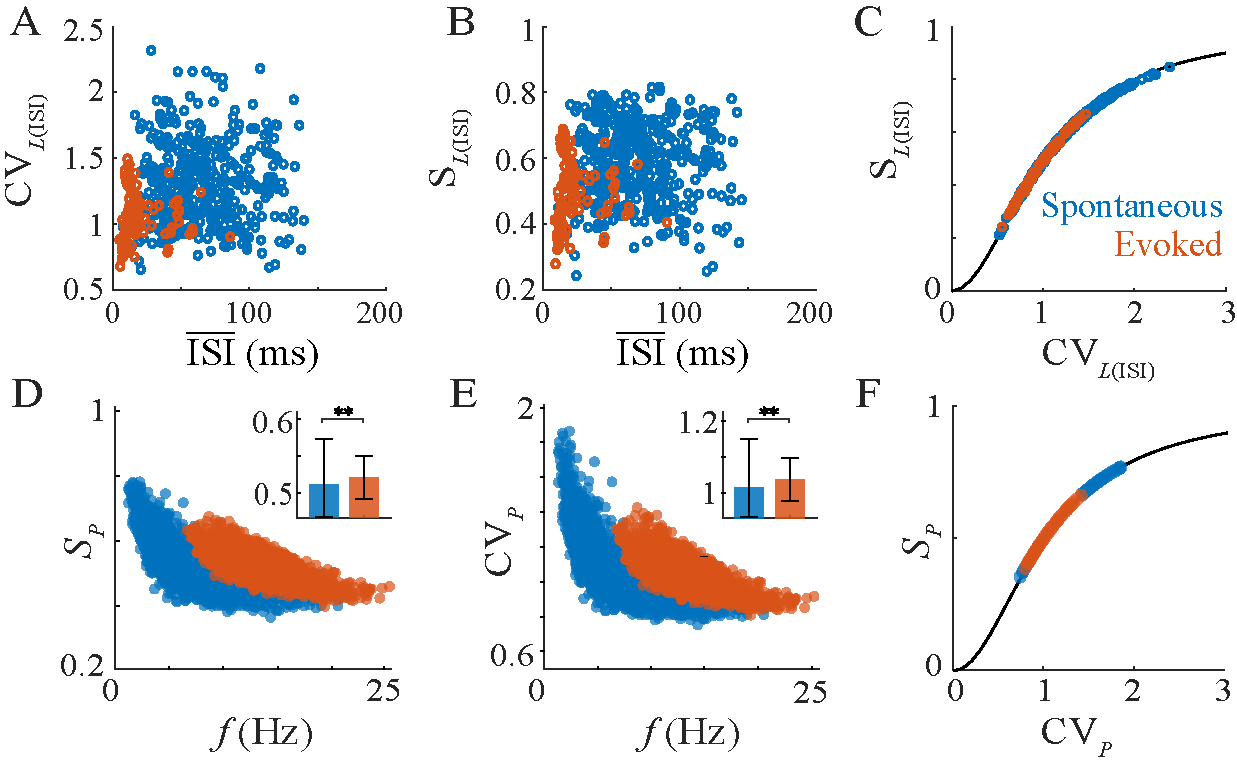
\includegraphics[scale=0.5]{figures/FigureS1.pdf}% Here is how to import EPS art

\caption{\textbf{Complementary CV estimators on the V1 dataset.}  (\textbf{A--C}) $S$--CV relationship using the inter-spike-interval $\mathrm{CV}_{ISI}$ and corresponding $S(\mathrm{ISI})$, vs.\ mean firing rate (A,B) and vs.\ each other (C).  (\textbf{D--F}) Same relationship using per-trial population $\mathrm{CV}_P$ and $S_P$.  Blue: spontaneous; orange: evoked; black curves: identity $S = \mathrm{CV}^2/(1+\mathrm{CV}^2)$.  All three estimators ($\mathrm{CV}_L$ in main Fig.~2, $\mathrm{CV}_{ISI}$ here, $\mathrm{CV}_P$ here) trace the same algebraic relation.}
\end{figure}

\setcounter{figure}{1}
\begin{figure}[H]
\centering 
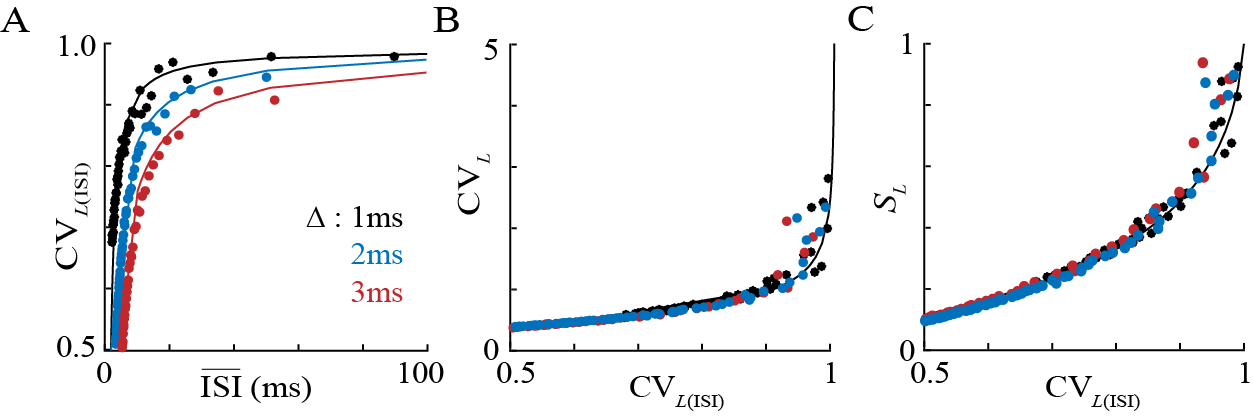
\includegraphics[scale=0.58]{figures/FigureS2.jpg}% Here is how to import EPS art

\caption{\textbf{$\mathrm{CV}_{L(ISI)}$--$S_L$ relationship for Poisson processes with absolute refractory period.}  Refractory periods $\Delta = 1, 2, 3$\,ms (black, dark gray, light gray dots).  (\textbf{A}) $\bar{ISI}$ vs.\ $\mathrm{CV}_{L(ISI)}$, with analytical curve (black line).  (\textbf{B}) $\mathrm{CV}_{L(ISI)}$ vs.\ instantaneous-rate $\mathrm{CV}_L$ (monotonic).  (\textbf{C}) $S_L$ vs.\ $\mathrm{CV}_{L(ISI)}$ matches the derived identity (black line).}
\end{figure}


\setcounter{figure}{2}
\begin{figure}[H]
\centering
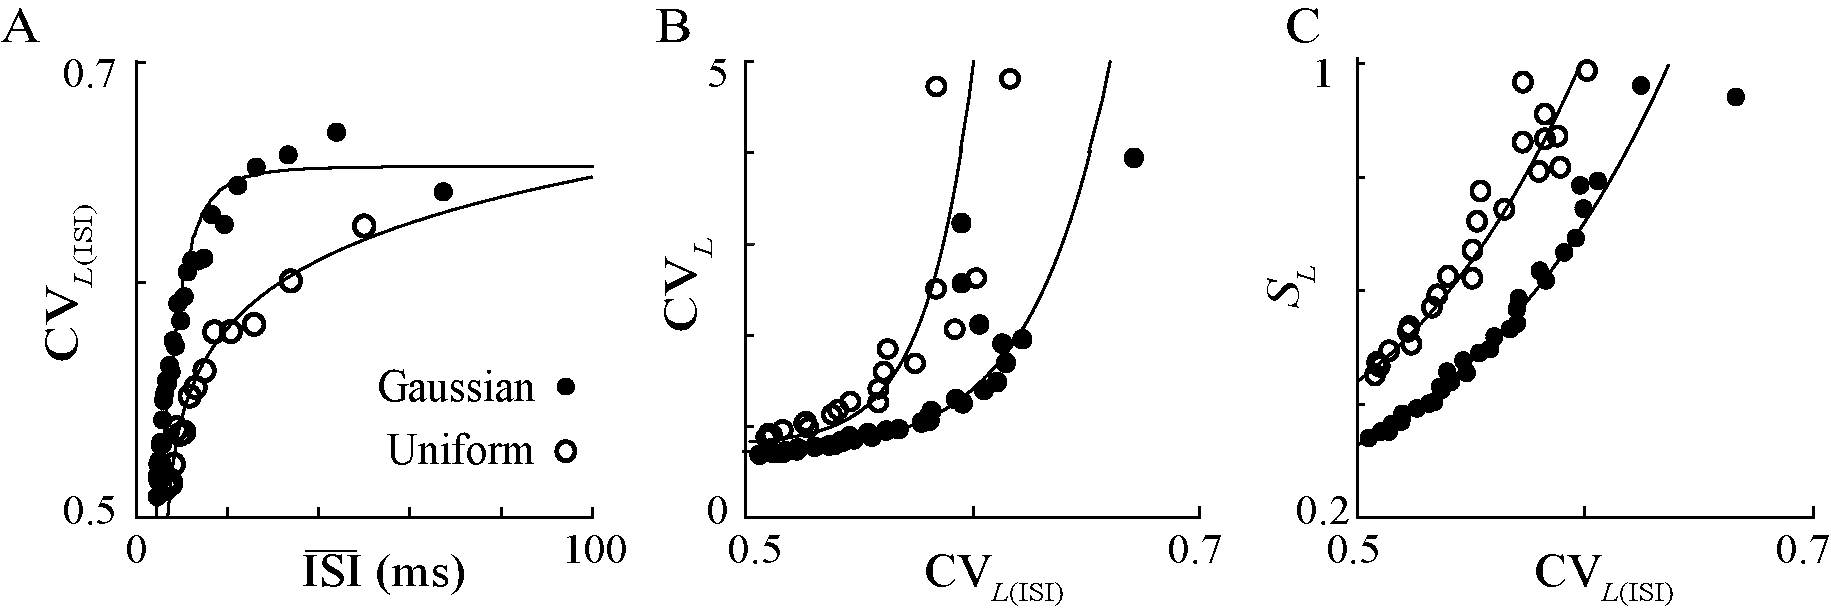
\includegraphics[width=0.95\textwidth]{figures/FigureS3.pdf}
\caption{\textbf{Per-trial population CV ($\mathrm{CV}_P$) and sparseness ($S_P$) on the V1 dataset (complementary projection to main-text Fig.~2).}  Each dot is one trial ($n=3200$ per condition); spontaneous (blue), evoked (orange).  (\textbf{A}) $S_P$ vs.\ per-trial mean firing rate.  (\textbf{B}) $\mathrm{CV}_P$ vs.\ mean firing rate; dashed line marks the unbounded-exponential limit $\mathrm{CV}=1$.  (\textbf{C}) $S_P$--$\mathrm{CV}_P$ scatter follows the identity $S = \mathrm{CV}^2/(1+\mathrm{CV}^2)$ (black curve).  In the $\mathrm{CV}_P$ view spontaneous and evoked overlap strongly ($\mathrm{CV}_P$ median $1.02$ vs.\ $1.04$, Cliff's $\delta=-0.05$) and the separation is along the firing-rate axis (median $6.5$ vs.\ $13.0$\,Hz, $\delta=-0.82$); the lifetime-CV view (main Fig.~2) instead separates them along the variability axis ($\mathrm{CV}_L$ $\delta=+0.34$).}
\label{fig:S_CVP}
\end{figure}



\setcounter{figure}{3}
\begin{figure}[H]
\centering
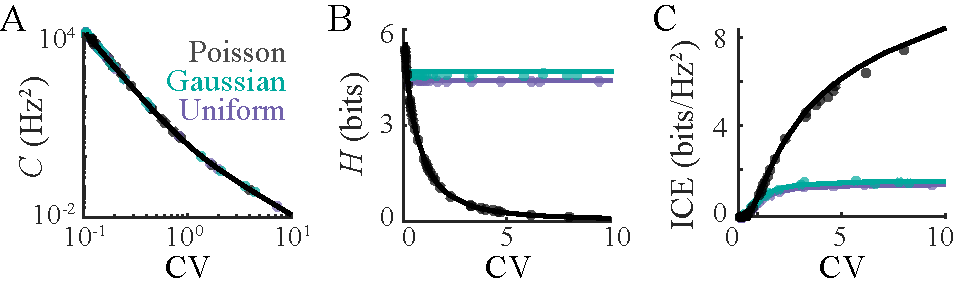
\includegraphics[width=0.85\textwidth]{figures/FigureS4.pdf}
\caption{\textbf{Distributional robustness check: ICE--CV monotonicity across three non-Gibbs families.}  Within-family ordering only; absolute ICE values are not comparable across families (Poisson: discrete Shannon entropy; Gaussian/Uniform: differential entropy).  (\textbf{A}) Signal energy $C=\mathbb{E}[r^2]$ vs.\ CV.  (\textbf{B}) Entropy $H$ vs.\ CV (Gaussian and Uniform constant because $\sigma$ is fixed; Poisson decreases).  (\textbf{C}) ICE $= H/\mathbb{E}[r^2]$ vs.\ CV: all three families yield strictly increasing ICE.  Dots: Monte-Carlo validation ($10^5$ samples).}
\label{fig:S_distribution_robustness}
\end{figure}

\setcounter{figure}{4}
\begin{figure}[H]%H为当前位置，!htbtb为忽略美学标准，htbp为浮动图形
\centering %图片居中
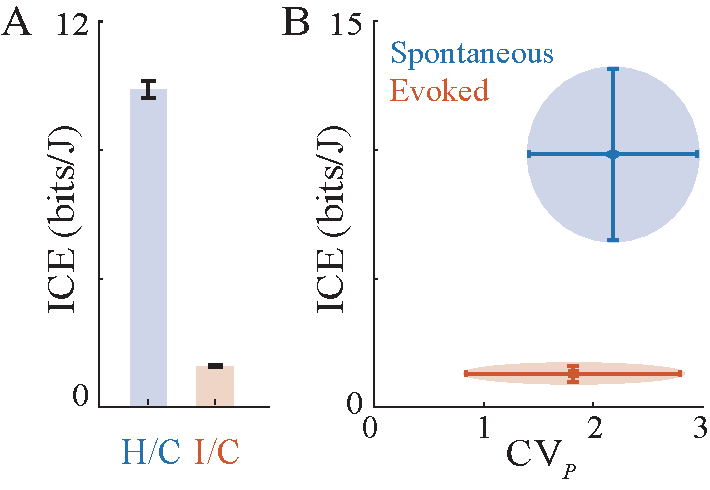
\includegraphics[width=0.34\textwidth]{figures/FigureS5.pdf} %插入图片，[]中设置图片大小，{}中是图片文件名
\caption{
Positive correlation between the coefficient of variation (CV) and coding efficiency (ICE) validated by experimental data on a population scale.
(A) Comparison of entropy-based efficiency (H/C) and information-based efficiency (I/C), showing consistent trends.
(B) ICE as a function of population CV ($CV_P$) for spontaneous and evoked activity, demonstrating that higher variability is associated with higher efficiency across conditions.
}
\end{figure}


\setcounter{figure}{5}
\begin{figure}[H]%H为当前位置，!htbtb为忽略美学标准，htbp为浮动图形
\centering %图片居中
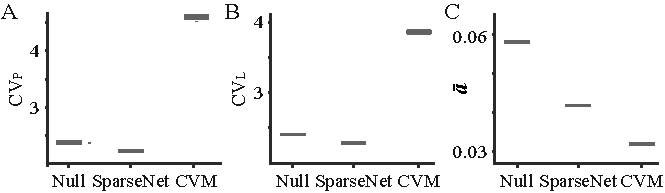
\includegraphics[width=0.65\textwidth]{figures/FigureS6.pdf} %插入图片，[]中设置图片大小，{}中是图片文件名
\caption{\textbf{Population statistics across the three sparse-coding models} (Null, SparseNet with Cauchy prior, CV-max; all pairwise $p<0.0001$).  (\textbf{A})~$\mathrm{CV}_P$: CVM ($2.72$) $>$ Null ($2.39$) $>$ SparseNet ($2.25$).  (\textbf{B})~$\mathrm{CV}_L$: CVM ($2.61$) $>$ Null ($2.41$) $>$ SparseNet ($2.29$).  (\textbf{C})~Mean activation $\bar{a}$: SparseNet ($0.042$) $<$ CVM ($0.050$) $<$ Null ($0.058$).  (\textbf{D})~Reconstruction error $\mathrm{RE}$: CVM ($0.625$) $\approx$ Null ($0.611$) $<$ SparseNet ($0.702$).  SparseNet's lower mean activation does not translate into higher ICE because its RE is elevated (cf.\ main-text Fig.~6F).}
\end{figure}

\setcounter{figure}{6}
\begin{figure}[H]
\centering
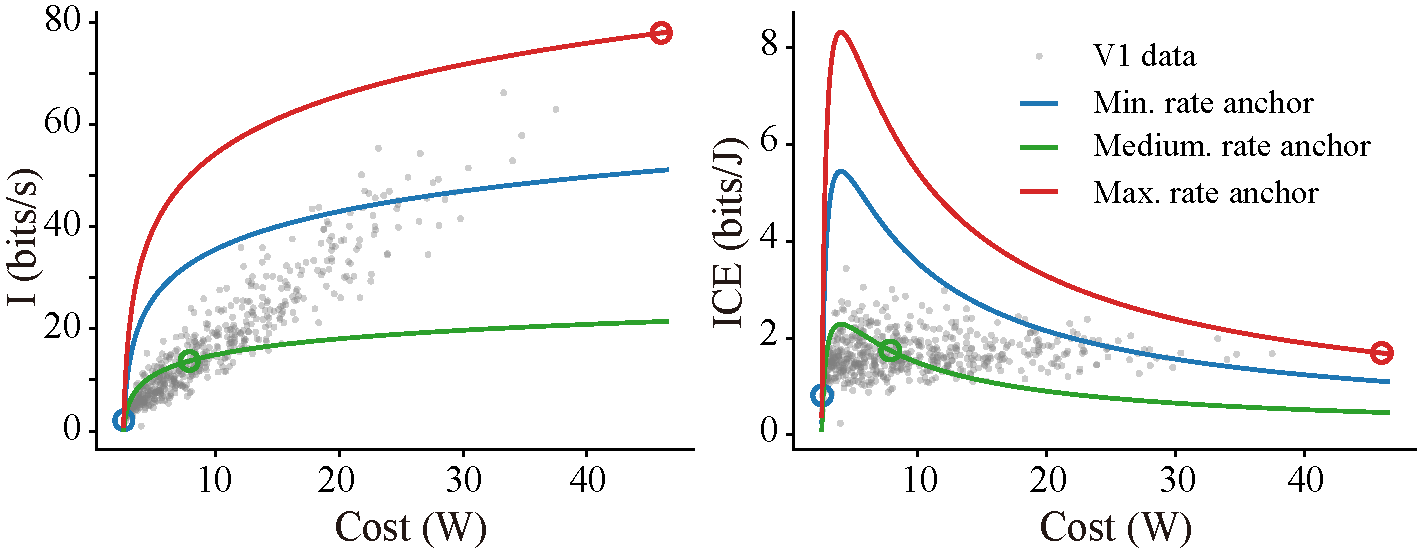
\includegraphics[width=\textwidth]{figures/FigureS7.pdf}
\caption{\textbf{Sensitivity of the main-text Fig.~5 Gibbs manifold to the $R_0$ anchor choice} (V1 pool, $n=564$).  Grey dots: V1 per-neuron data; colored curves: Gibbs-optimal manifold $I^{\star}(C)=(R_0/\ln 2)[1+\ln((C-C_0)/C_1)]$ under three anchors (open circles): minimum-rate $\Rightarrow R_0=6.13$ (upper envelope), median-rate $\Rightarrow R_0=2.58$ (used in main-text Fig.~5C; central trend), maximum-rate $\Rightarrow R_0=9.36$ (loose ceiling).  (\textbf{Left}) $I$--$C$.  (\textbf{Right}) $\mathrm{ICE}$--$C$.  Topology (data concavity, rank order, $\mathrm{ICE}>\beta$) is anchor-invariant; only the absolute scale and data-to-manifold gap depend on the anchor (full numbers in Table~\ref{tab:anchor-summary}).}
\label{fig:S6-anchor}
\end{figure}

\setcounter{figure}{7}
\begin{figure}[H]
\centering
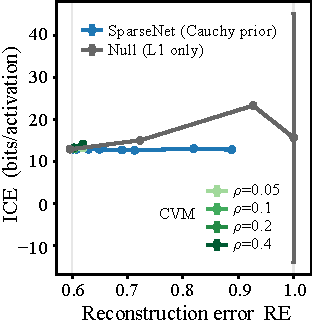
\includegraphics[width=0.85\textwidth]{figures/FigureS8.pdf}
\caption{\textbf{CV-max ICE--RE Pareto curves and matched-baseline ablation.}  Each marker: (method, regularization) configuration averaged over 3 seeds.  CVM (green ramp): four sub-curves indexed by adaptive ratio $\rho\in\{0.05,0.10,0.20,0.40\}$, each sweeping the absolute-RE target $\tau\in\{0.40,0.50,0.55,0.60\}$.  Null (grey): L1 weight $\lambda\in[10^{-4},5\!\cdot\!10^{-2}]$.  SparseNet (blue): Cauchy weight $\alpha_s\in[0.05,10]$.  Dashed line: matched-RE comparison at $\mathrm{RE}=0.60$.  CVM sub-curves lie at or above Null throughout the displayed range, confirming that the main-text Fig.~6F ICE advantage is not specific to one regularization weight.  SparseNet does not reach $\mathrm{RE}<0.602$ at any $\alpha_s$ tested.  Plot cropped at $\mathrm{RE}\ge 0.60$ for legibility; under-regularized Null configurations at lower RE inflate $\bar{a}$ by up to $2.5\times$ and sit below the headline Null point in ICE (full numbers in main text).}
\label{fig:S7-cvm-ablation}
\end{figure}

\setcounter{figure}{8}
\begin{figure}[H]%H为当前位置，!htbtb为忽略美学标准，htbp为浮动图形
\centering %图片居中
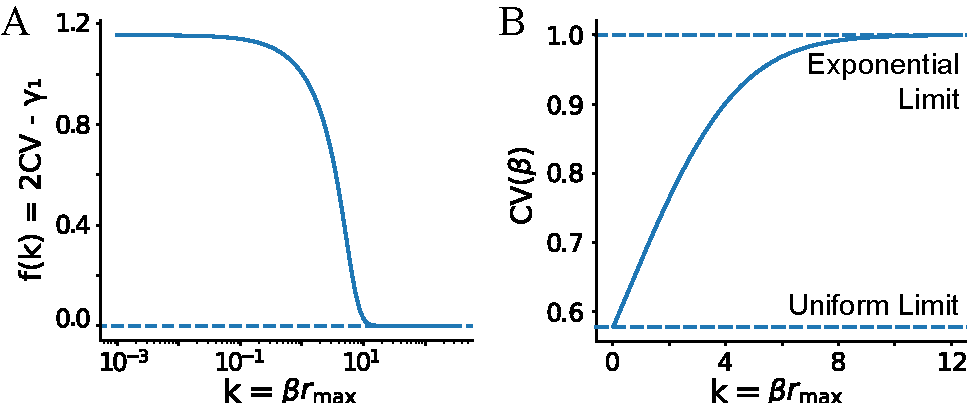
\includegraphics[width=0.48\textwidth]{figures/FigureS9.pdf} %插入图片，[]中设置图片大小，{}中是图片文件名

\caption{\textbf{Analytical reduction and numerical verification of CV--$\beta$ monotonicity for the truncated-exponential optimal code.}  (\textbf{A}) Auxiliary $f(k)=2\,\mathrm{CV}(k)-\gamma_{1}(k)$ is numerically positive on a dense grid of $k=\beta r_{\max}>0$, supporting the inequality equivalent to $\frac{d}{d\beta}\log\mathrm{CV}>0$ (combined with the reduction in Section~1.3.5; we do not claim a closed-form positivity proof).  (\textbf{B}) The optimal CV--$k$ curve rises from the uniform limit $1/\sqrt{3}$ to the exponential limit $1$.}
\label{fig:S9-trunc-exp-monotone}
\end{figure}

\setcounter{figure}{9}
\begin{figure}[H]%H为当前位置，!htbtb为忽略美学标准，htbp为浮动图形
\centering %图片居中
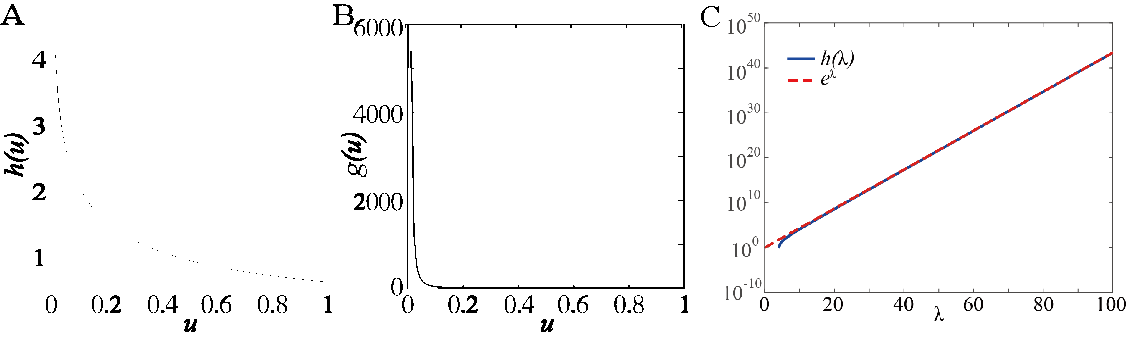
\includegraphics[width=0.74\textwidth]{figures/FigureS10.pdf} %插入图片，[]中设置图片大小，{}中是图片文件名

\caption{\textbf{Numerical validations for supplementary proofs.}  (\textbf{A,B}) $h(u)$ and $g(u)$ are positive on $u\in(0,1)$.  (\textbf{C}) $h(\lambda)$ (blue) lies below $e^\lambda$ (dashed red) on $\lambda\in(0,100)$, supporting the bound used in Theoretical Framework Section B.}
\end{figure}

\setcounter{figure}{10}
\begin{figure}[H]
\centering
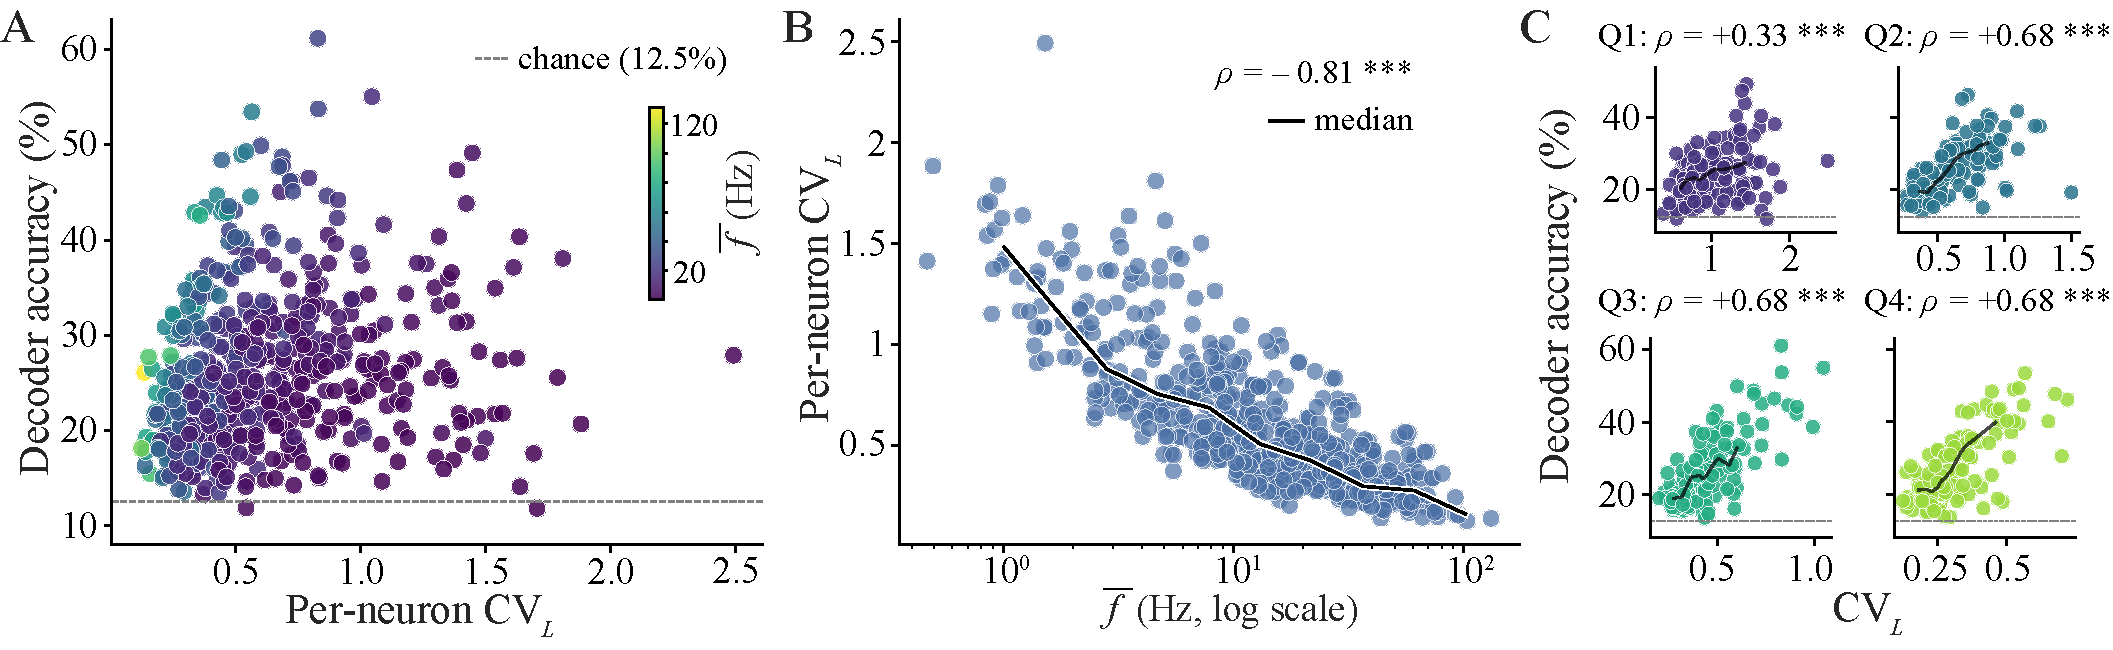
\includegraphics[width=\textwidth]{figures/FigureS11.pdf}
\caption{\textbf{FR-controlled per-neuron decoder validation of the CV--reliability link on macaque V1} ($N=564$ neurons, 5 v1v2-1 sessions).  Per-neuron 8-class LDA on per-trial spike counts (1.28\,s drifting-grating window; 10-fold stratified CV; main-text Methods, ``Per-neuron decoder analysis'').  Three-panel causal chain: raw relationship $\to$ confounder revealed $\to$ FR control.  (\textbf{A}) Pooled scatter of decoder accuracy vs $\mathrm{CV}_L$, color-coded by mean firing rate; dashed line is 8-stim chance ($12.5\%$).  Raw $\rho_{\mathrm{raw}}=+0.29$ ($p=10^{-12}$); FR-partialled $\rho_{\,|\,\mathrm{FR}}=+0.68$ ($p=10^{-78}$).  (\textbf{B}) Confounder: $\mathrm{CV}_L$ vs FR (log scale) with running median (black); $\rho=-0.81$ ($p<10^{-100}$).  Both $\mathrm{CV}_L$ and FR positively predict accuracy, so this negative inter-correlation suppresses the raw $\rho$ in A.  (\textbf{C}) Within each FR quartile (Q1: 0.5--6.5\,Hz, Q2: 6.5--15\,Hz, Q3: 15--29\,Hz, Q4: 29--131\,Hz), higher-$\mathrm{CV}_L$ neurons achieve higher accuracy ($\rho_{\mathrm{Q1}}=+0.33$, $\rho_{\mathrm{Q2}}=+0.68$, $\rho_{\mathrm{Q3}}=+0.68$, $\rho_{\mathrm{Q4}}=+0.68$; all $p<10^{-4}$).  Per-session: within-session partial $\rho$ ranges $+0.54$ to $+0.83$ across the 5 sessions (all $p<10^{-9}$); Fisher-combined $\rho_{\mathrm{meta}}=+0.72$ ($p=10^{-100}$).  Significance: $^{*}p<0.05$, $^{**}p<0.01$, $^{***}p<0.001$.}
\label{fig:S11-decoder-vs-CV}
\end{figure}

\newpage


\section{Supplementary Tables}

\begin{table}[h!]
\centering
\small
\caption{\textbf{Bookkeeping of information--cost quantities used across this study.}  Columns: the three measurement contexts; rows: the actual quantity computed, its interpretation, and its role.  Operational details (binning, estimator, units) are in Methods.}
\label{tab:bookkeeping}
\begin{tabular}{p{2.2cm}p{3.4cm}p{3.4cm}p{3.4cm}}
\toprule
 & \textbf{Theory (derivation)} & \textbf{Empirical (evoked)} & \textbf{Empirical (spontaneous)} \\
\midrule
\textbf{Quantity computed} &
$H(r)/C$, identified with $I(s;r)/C$ under $H(r|s)\approx 0$ &
$I(s;r)/C$ via Direct Method (models and V1 evoked) &
$H(r)/C$ (no stimulus defined; $I(s;r)$ undefined) \\
\addlinespace
\textbf{Interpretation} &
Closed-form Gibbs manifold; benchmark against which empirical points are read &
Deployed information per unit cost.  In V1, the noise-entropy fraction $\bar\rho\approx 0.85$ is reported separately so the gap $H-I$ is explicit &
Coding readiness: the maximum information the network \emph{could} transmit at the current metabolic state \\
\addlinespace
\textbf{Role} &
Normative target &
Test of within-system ICE--CV monotonicity and manifold alignment &
Readiness measure used in resting-state comparisons \\
\bottomrule
\end{tabular}
\end{table}

\begin{table}[h!]
\centering
\caption{\textbf{V1 spontaneous vs.\ evoked statistics (per-neuron lifetime metrics, $N=159$).}  Per-neuron lifetime CV ($\mathrm{CV}_L$), Vinje--Gallant bias-corrected sparseness ($S_L$), and mean firing rate, paired across the same neurons.  Columns: condition medians, median paired difference $\Delta_{\mathrm{med}}$ (spontaneous $-$ evoked) with 10{,}000-resample bootstrap $95\%$ CI, Wilcoxon signed-rank statistic and two-sided $p$-value, and Cliff's $\delta$.  Spontaneous exceeds evoked on $\mathrm{CV}_L$ and $S_L$ (Cliff's $\delta\approx +0.34$); the complementary per-trial population view is in Supplementary Fig.~S3.  Dataset: CRCNS \texttt{v1v2-1}, session \texttt{105l001p16}.}
\begin{tabular}{lcccccc}
\toprule
Quantity & median$_{\mathrm{spon}}$ & median$_{\mathrm{evk}}$ & $\Delta_{\mathrm{med}}$ & $95\%$ CI & $W$, $p$ & Cliff's $\delta$ \\
\midrule
$\mathrm{CV}_L$        & $0.822$  & $0.632$  & $+0.179$ & $[+0.143,\,+0.205]$ & $2027$, $9.2\!\times\!10^{-14}$ & $+0.339$ \\
$S_L$                  & $0.403$  & $0.286$  & $+0.106$ & $[+0.085,\,+0.123]$ & $1741$, $2.0\!\times\!10^{-15}$ & $+0.339$ \\
mean rate (Hz)         & $4.89$   & $9.08$   & $-3.70$  & $[-4.72,\,-2.90]$  & $795$,  $1.1\!\times\!10^{-21}$ & $-0.332$ \\
\bottomrule
\end{tabular}
\label{tab:fig2-stats}
\end{table}

\begin{table}[h!]
\centering
\caption{Summary of main symbols used in the manuscript.}
\begin{tabular}{ll}
\hline
\textbf{Symbol} & \textbf{Description} \\
\hline
$r$ & Firing rate (scalar variable) \\
$p(r)$ & Firing-rate distribution \\
$c(r)$ & Metabolic cost function \\
$C$ & Metabolic budget (expected cost) \\
$H(r)$ & Shannon entropy of the rate distribution \\
$\mathrm{ICE}$ & Information--cost efficiency: $H/C$ \\
$\beta$ & Lagrange multiplier (marginal efficiency / inverse temperature) \\
$p_\beta(r)$ & Gibbs-optimal firing-rate distribution \\
$r_{\max}$ & Upper bound on firing rate \\
$\mu,\sigma^2$ & Mean and variance of $r$ \\
$\mathrm{CV}=\sigma/\mu$ & Coefficient of variation \\
$S$ & Lifetime sparseness: $S = CV^2 / (1 + CV^2)$ \\
$W$ & Synaptic weight matrix in recurrent model \\
$E,I$ & Excitatory and inhibitory populations \\
\hline
\end{tabular}
\label{table:symbols}
\end{table}


\begin{table}[H]
\centering
\caption{Summary of detailed parameters for the single-neuron leaky integrate-and-fire simulations in Result Section 3.2.}
\label{tab:lif-params}
\begin{tabular}{lll}
\hline
\textbf{Symbol} & \textbf{Description} & \textbf{Value} \\
\hline
$\eta$        & Learning rate & 0.0002 \\
$\alpha$      & Decay term (proportional to $\eta$) & $0.25 \times \eta$ \\
$\tau_{\text{plasticity}}$ & Time window of the learning rule & 20 ms \\
$dt$          & Simulation time step & 0.1 ms \\
$\text{duration}$ & Duration of a single run & 1500 ms \\
$N_{\text{runs}}$ & Number of consecutive runs & 80 \\
$t_{\text{ref}}$  & Refractory period & 5 ms \\
$g_{\text{Ex}}$   & Excitatory synaptic conductance scaling (relative to leak, $g_{\text{leak}}=10$ nS) & 0.014 \\
$g_{\text{In}}$   & Inhibitory synaptic conductance scaling & 0.035 \\
$V_{\text{rest}}$ & Resting potential & -60 mV \\
$V_{\text{th}}$   & Spike threshold potential & -50 mV \\
$\tau_{\text{mem}}$ & Membrane time constant & 20 ms \\
$E_{\text{AMPA}}$ & Excitatory reversal potential & 0 mV \\
$E_{\text{GABA}}$ & Inhibitory reversal potential & -80 mV \\
$\tau_{\text{Ex}}$ & Excitatory synaptic time constant & 5 ms \\
$\tau_{\text{In}}$ & Inhibitory synaptic time constant & 10 ms \\
\hline
\end{tabular}
\end{table}

\begin{table}[H]
\centering
\caption{Summary of mathematical symbols and their corresponding default values used in the network model in Section 4.1.}
\label{tab:network-params}
\begin{tabular}{lll}
\hline
\textbf{Symbol} & \textbf{Description} & \textbf{Value} \\
\hline
$\lambda$    & Membrane leak constant & 50 \\
$\Delta t$   & Time step for simulation & 0.0001 s \\
$N_x$        & Input signal dimensionality & 3 \\
$N_E$        & Number of excitatory neurons & 300 \\
$N_I$        & Number of inhibitory neurons & 75 \\
$F_{nj}$     & Feedforward weight from input $j$ to neuron $n$ & Random \& normalized \\
$\Omega^{EE}$ & Recurrent weights: Excitatory $\rightarrow$ Excitatory & Initialized weak \\
$\Omega^{II}$ & Recurrent weights: Inhibitory $\rightarrow$ Inhibitory & Initialized weak \\
$\Omega^{EI}$ & Recurrent weights: Excitatory $\rightarrow$ Inhibitory & Initialized weak \\
$\Omega^{IE}$ & Recurrent weights: Inhibitory $\rightarrow$ Excitatory & Initialized weak \\
$T_E$        & Threshold of excitatory neurons & Half the norm of FF weights \\
$T_I$        & Threshold of inhibitory neurons & Same as $T_E$ \\
$\lambda_E$  & Integration time constant for E neurons & $\lambda \times 6$ \\
$\lambda_I$  & Integration time constant for I neurons & $\lambda \times 1$ \\
$\eta_F$     & Learning rate for feedforward weights & $1 \times 10^{-5}$ \\
$\eta_\Omega$& Learning rate for recurrent weights & $1 \times 10^{-4}$ \\
$\mu$        & Regularization coefficient in cost function & 0.002 \\
$N_{\text{it}}$ & Number of training iterations & $2^{23}$ \\
$N_{\text{time}}$ & Number of time steps per iteration & 1000 \\
\hline
\end{tabular}
\end{table}

\newpage
\bibliographystyle{plain}
\bibliography{sn-bibliography}

\end{document}